\documentclass[12pt]{article}
\usepackage[utf8]{inputenc}
\usepackage[russian]{babel}
\usepackage [left=30 mm, top=30 mm, right=30 mm, bottom=20mm, nohead, footskip=10 mm] {geometry}
%\usepackage{pscyr}
\usepackage{multicol}
\usepackage{lipsum}
\usepackage{mwe}
\usepackage[T2A]{fontenc}
\usepackage{amsmath}
\usepackage{amssymb}
\usepackage{graphicx}
\graphicspath{{src/}}
\usepackage{listings}   
\usepackage{hyperref}
\usepackage{fancyhdr}
%\usepackage{algorithm}
\usepackage{algpseudocode}
\usepackage{indentfirst}
\usepackage{listings}
\usepackage{caption}
\usepackage{hyperref}
\addto\captionsrussian{\def\refname{Список источников}}
\hypersetup{
    colorlinks=true,
    linkcolor=blue,
    filecolor=magenta,      
    urlcolor=cyan,
}
\usepackage{float}%"Плавающие" картинки
\hypersetup{
    colorlinks=true,
    linkcolor=blue,
    filecolor=magenta,      
    urlcolor=cyan,
    pdftitle={Sharelatex Example},
    bookmarks=true,
    pdfpagemode=FullScreen,
}
\usepackage{wrapfig}%Обтекание фигур (таблиц, картинок и прочего)

\parindent=24pt


\begin{document}

\begin{center}
\hfill \break
\large{МИНОБРНАУКИ РОССИИ} \\
\hfill \break
\small {ФЕДЕРАЛЬНОЕ ГОСУДАРСТВЕННОЕ БЮДЖЕТНОЕ ОБРАЗОВАТЕЛЬНОЕ УЧРЕЖДЕНИЕ }\\
\small { ВЫСШЕГО ПРОФЕССИОНАЛЬНОГО ОБРАЗОВАНИЯ  } \\
\hfill \break
\normalsize {\textbf{ <<САНКТ-ПЕТЕРБУРГСКИЙ ПОЛИТЕХНИЧЕСКИЙ УНИВЕРСИТЕТ } }\\
{\normalsize {\textbf { ПЕТРА ВЕЛИКОГО>>}}} \\
\hfill \break
\large{Институт Компьютерных Наук и Кибербезопасности }\\
\hfill \break
\large{ Высшая школа технологий искуственного интелекта }\\
\hfill \break
Направление 02.03.01 Математика и Компьютерные Науки\\
\vskip 1cm
\large {Отчет по лабораторной работе №1:}
\vskip 0.2cm
\large {По дисциплине:}

\large{<<Алгоритмические основы компьютерной графики>>} \\
\hfill \break
\normalsize{Тема Работы:} \\
\hfill \break
\normalsize{<<Моделирование трехмерных объектов>>} \\
\thispagestyle {empty}

\hfill \break
\vskip 0.3cm
\vskip 1cm
\end{center}
\begin {tabular}{cccc}
\hspace{0.5cm}Обучающийся: &\underline {\hspace{3cm}} &  &Черепанов Михаил Дмитриевич\\\\
\hspace{0.5cm}Руководитель: &\underline {\hspace{3cm}} & &Курочкин Михаил Александрович\\\\
\end{tabular}
\vskip 0.5 cm
\hspace{9cm}\def \hrf#1{\hbox to#1{\hrulefill}}<<\hrf{2em}>>  \hrf{6em}  20\hrf{1em}~r.
\vskip 2cm
\begin {center} Санкт-Петербург 2024 \end{center}
\newpage
\tableofcontents
\newpage






\section*{Введение}
\addcontentsline{toc}{section}{Введение}
3D-моделирование – это процесс создания трёхмерной модели объекта. 3D-моделирование
широко используется в таких областях как компьютерная графика, разработка компьютерных игр, кино, мультипликация, инженерная графика, архитектура, дизайн.

Одной из задач 3D моделирования является построение реалистических моделей объектов
реального мира. Реалистичность модели определяется следующими параметрами:

1 Соответствие геометрической формы реальному объекту;

2 Соответствие материала модели материалу реального объекта с сохранением таких особенностей как цвет и текстура объекта.

В данной работе необходимо сделать модели трех объектов из реального мира в одной из программ, предоставляющих интерфейс для создания трехмерных моделей.




\newpage

\section{Постановка задачи}

\begin{itemize}
\item Ознакомиться с возможностями пакета Blender, позволяющими создавать реалистичные 3D-модели.

\item Выбрать три объекта реального мира, с наличием каких-либо индивидуальных особенностей (Оригинальной формы, налиичие дефектов).

\item Создать модели выбранных объектов с отражением геометрической формы и индивидуальных особенностей.

\item Предоставить пошаговое руководство пользователя по получению результата для каждой из моделей.
\end{itemize}

\newpage


\section{Описание программного продукта Blender}


Blender — профессиональное свободное и открытое программное обеспечение для создания трёхмерной компьютерной графики, включающее в себя средства моделирования, анимации, симуляции, монтажа видео, создания 2D-анимации. В настоящее время пользуется большой популярностью среди бесплатных 3D-редакторов в связи с его быстрым стабильным развитием и технической поддержкой.

Отличительной чертой Blender является то, что это ПО с открытым исходным кодом и сообщество разработчиков, использующих данную программу может предлагать разработчикам Blender возможные изменения в соответствии с запросами пользователей. Это позволило данной среде стать более интуитивно понятной и более легкой в обучении, чем аналоги.

Отличительные особенности интерфейса пользователя:


\begin{itemize}
\item Режимы редактирования. Два основных режима Объектный режим (Object mode) и Режим редактирования (Edit mode). Объектный режим в основном используется для манипуляций с индивидуальными объектами, в то время как режим редактирования — для манипуляций с фактическими данными объекта.

\item Широкое использование горячих клавиш. Большинство команд выполняется с клавиатуры. 

\item Управление рабочим пространством. Графический интерфейс Blender’а состоит из одного или нескольких экранов, каждый из которых может быть разделён на секции и подсекции.
\end{itemize}


\subsection{Начало работы с Blender}

При запуске программы открывается главное окно   Blender. Его можно разделить на 5 основных частей:

\vskip 1cm
{
    \centering
    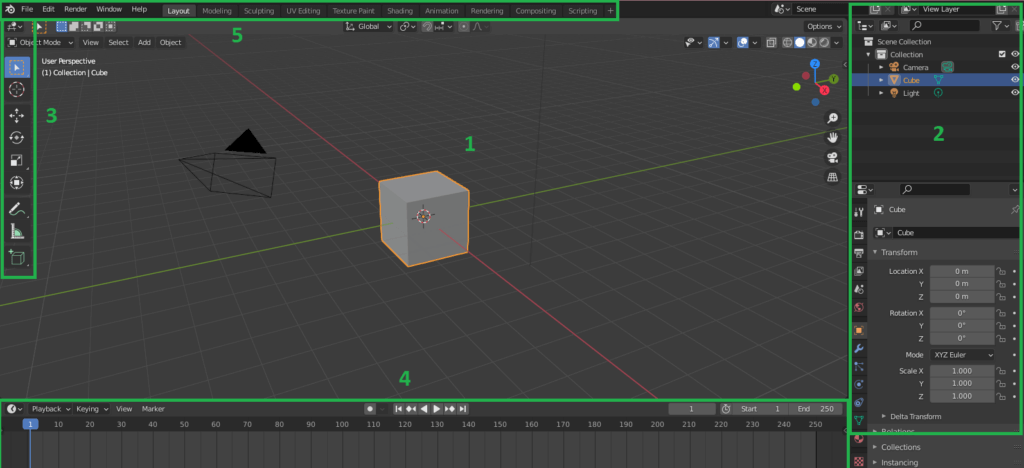
\includegraphics[width=1\linewidth]{гокно.png}
    \label{fig:i1}
}
\vskip 1cm


\begin{enumerate}
\item Основная рабочая область — это область трехмерного просмотра, в которой будет располагаться 3D-объект.
\item Панель настроек справа — это область, в которой можно менять свойства и параметры объекта.
\item Панель инструментов слева — в ней расположены иконки, с помощью которых можно выбрать нужный инструмент.
\item Временная шкала, необходимая для работы с анимацией.
\item Основное меню настроек файла.
\end{enumerate}

Далее расскажу об использовании каждой из этих частей подробнее.
\subsubsection{ Основная рабочая область }

Область известна также как 3D View. Она является основной рабочей зоной Blender. В ней происходит отображение проекции трехмерной сцены, и изначально в этой области появляется базовая фигура — куб. Он нужен, чтобы запустить рендеринг, посмотреть, как работают камера и источник света.

При создании нового файла по умолчанию в центре экрана будет расположен куб, как показано на скриншоте выше. Куб нужен для проверки, правильно ли работают все программные элементы, чтобы запустить рендеринг, посмотреть, как работают камера и источник света.

Куб можно заменить на другие стандартные объекты: окружность, сферу, цилиндр или конус. Также можно загрузить собственные объекты. Чтобы добавить объект в Blender, используйте сочетание клавиш Shift+A, чтобы открыть меню Add и выбрать нужную фигуру.

\vskip 1cm
{
    \centering
    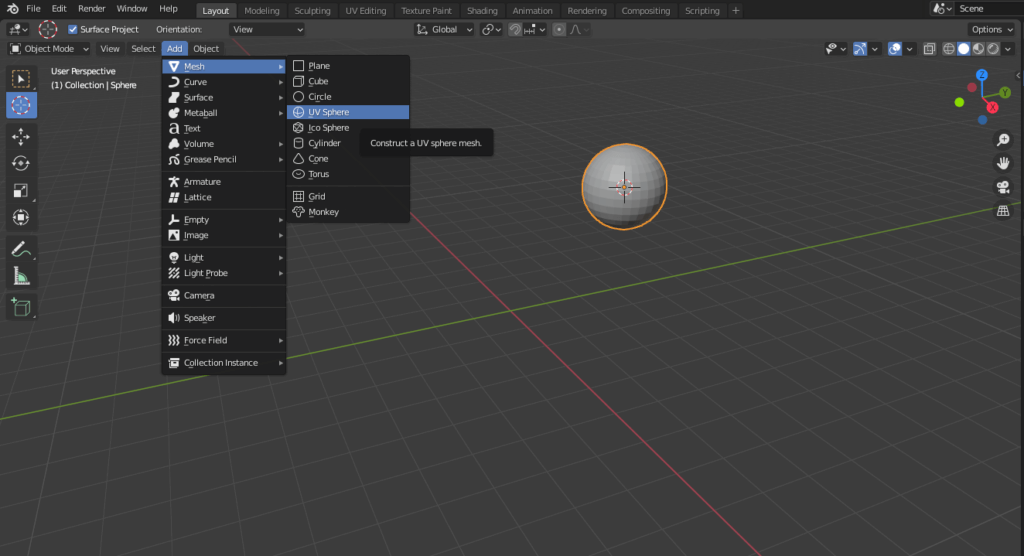
\includegraphics[width=1\linewidth]{добавление_объекта.png}
    \label{fig:i1}
}
\vskip 1cm

\subsubsection{ Боковая панель свойств }

Позволяет менять настройки (свойства) сцены и объектов. Из-за большого количества они разбиты на несколько групп. Переключаться между группами можно с помощью панели с иконками слева от свойств. Здесь можно управлять:

положением объекта (куба по умолчанию).
освещением.
положением камеры относительно объекта.
Открыть или закрыть боковую панель свойств можно с помощью клавиши N.

\vskip 1cm
{
    \centering
    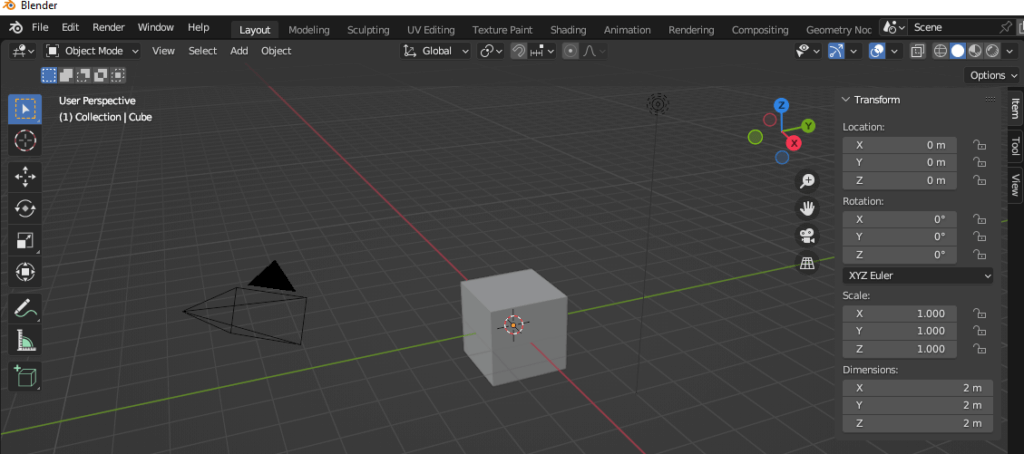
\includegraphics[width=1\linewidth]{панель_свойств.png}
    \label{fig:i1}
}
\vskip 1cm

\subsubsection{ Панель инструментов}

В панели инструментов находятся иконки всех доступных инструменты для моделирования, текстурирования и анимации. Вызвать ее можно с помощью клавиши T.



\vskip 1cm
{
    \centering
    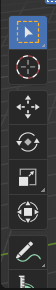
\includegraphics[width=0.07\linewidth]{панель_инструментов.png}
    \label{fig:i1}
}
\vskip 1cm

В зависимости от того, в каком режиме работы находится пользователь, на панели будут разные инструменты. Таким образом, пользователи могут легко переключаться между различными наборами, не теряя времени на поиск нужной функции.





\subsubsection{ Временная шкала}
Временная шкала или таймлайн отображают кадры анимации, а цветная полоса показывает текущий выбранный кадр. По умолчанию это всегда первый кадр. Таймлайн позволяет управлять временем в анимации, а также добавлять и удалять ключевые кадры для создания плавных анимационных переходов.


\subsubsection{ Основное меню}
С его помощью можно загрузить, сохранить или начать новый проект, сбросить настройки, рендерить проект и найти дополнительную информацию по программе.









\newpage
\section{Описание объектов моделирования}

\subsection{Объект № 1}

{\bf Наименование:} 

Клапан для воды.

{\bf Фото объекта:}

\vskip 1cm
{
    \centering
    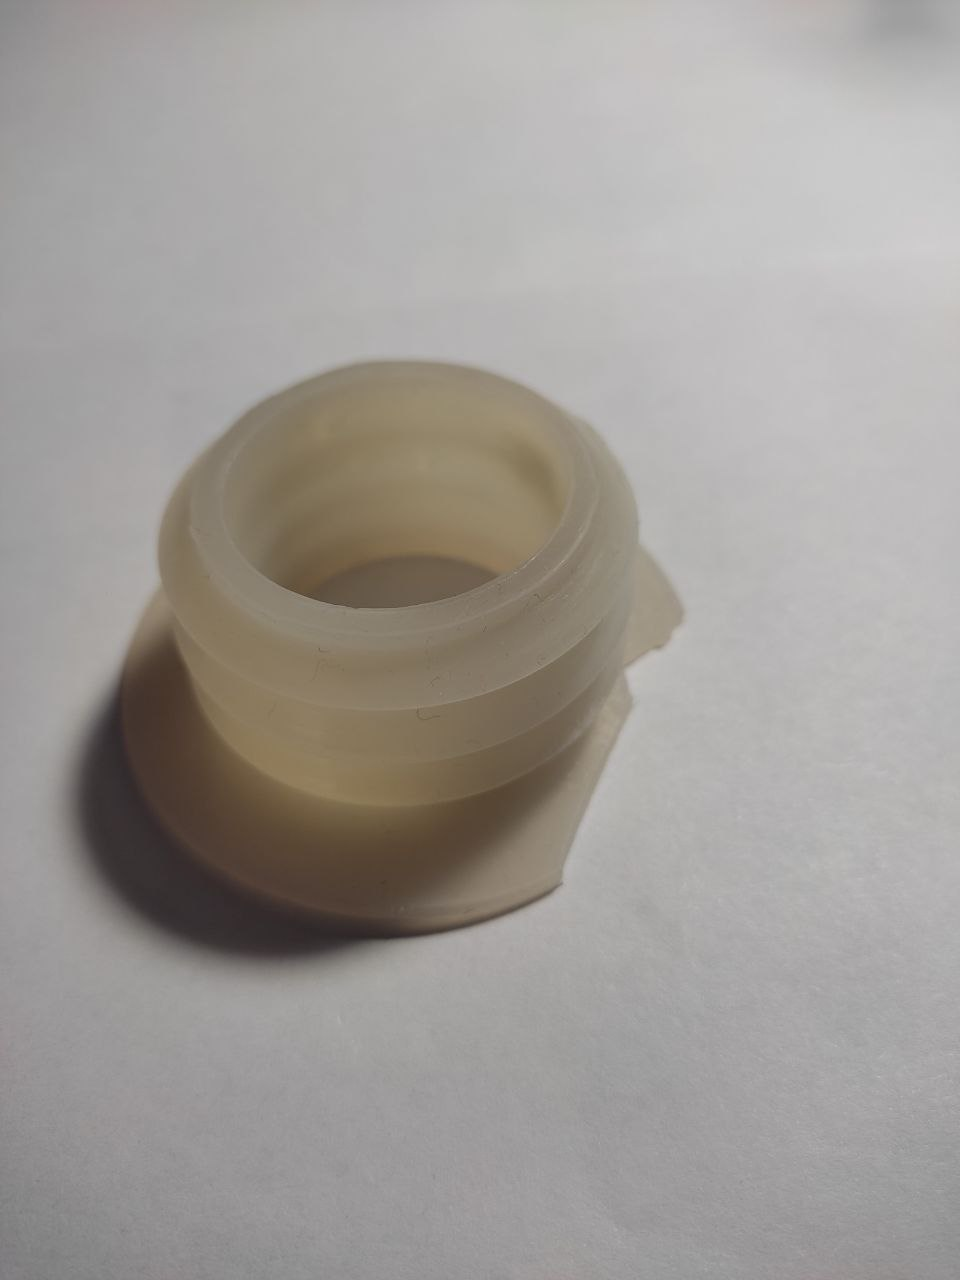
\includegraphics[width=0.6\linewidth]{клапан_норм_фото.jpeg}
    \label{fig:i1}
}
\vskip 1cm
{\bf Свойства объекта, которые необходимо отразить}

Циллиндрическая форма клапана с тремя дискообразными выступами и основанием.

Цвет объекта - серый.

В основании клапана имеется дефект в виде пореза.

\subsection{Объект № 2}

{\bf Наименование:} 

Дверной ключ.

{\bf Фото объекта:}

\vskip 1cm
{
    \centering
    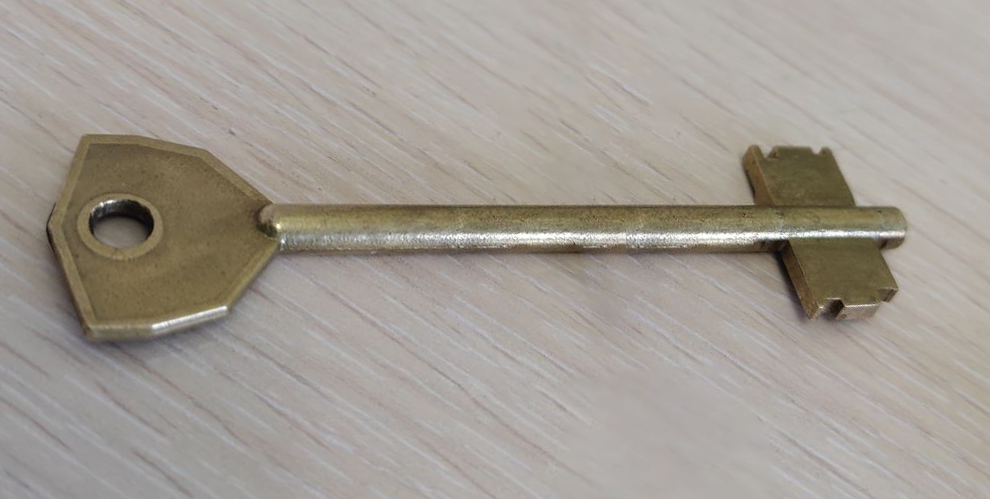
\includegraphics[width=1\linewidth]{ключ_без_дефекта.png}
    \label{fig:i1}
}
\vskip 1cm
{\bf Свойства объекта, которые необходимо отразить:}

Форма ключа, состоящая из ручки; основной части в виде циллиндра; рабочей части, которую вставляют в замочную скважену.

Цвет ключа - желтый, имеет металический блеск.

Рабочая часть имеет оригинальную форму, предназначенную для открытия конкретного замка.




    
 \subsection{Объект № 3}


{\bf Наименование:} 

Катушка с лейкопластырной лентой.

{\bf Фото объекта:}

\vskip 1cm
{
    \centering
    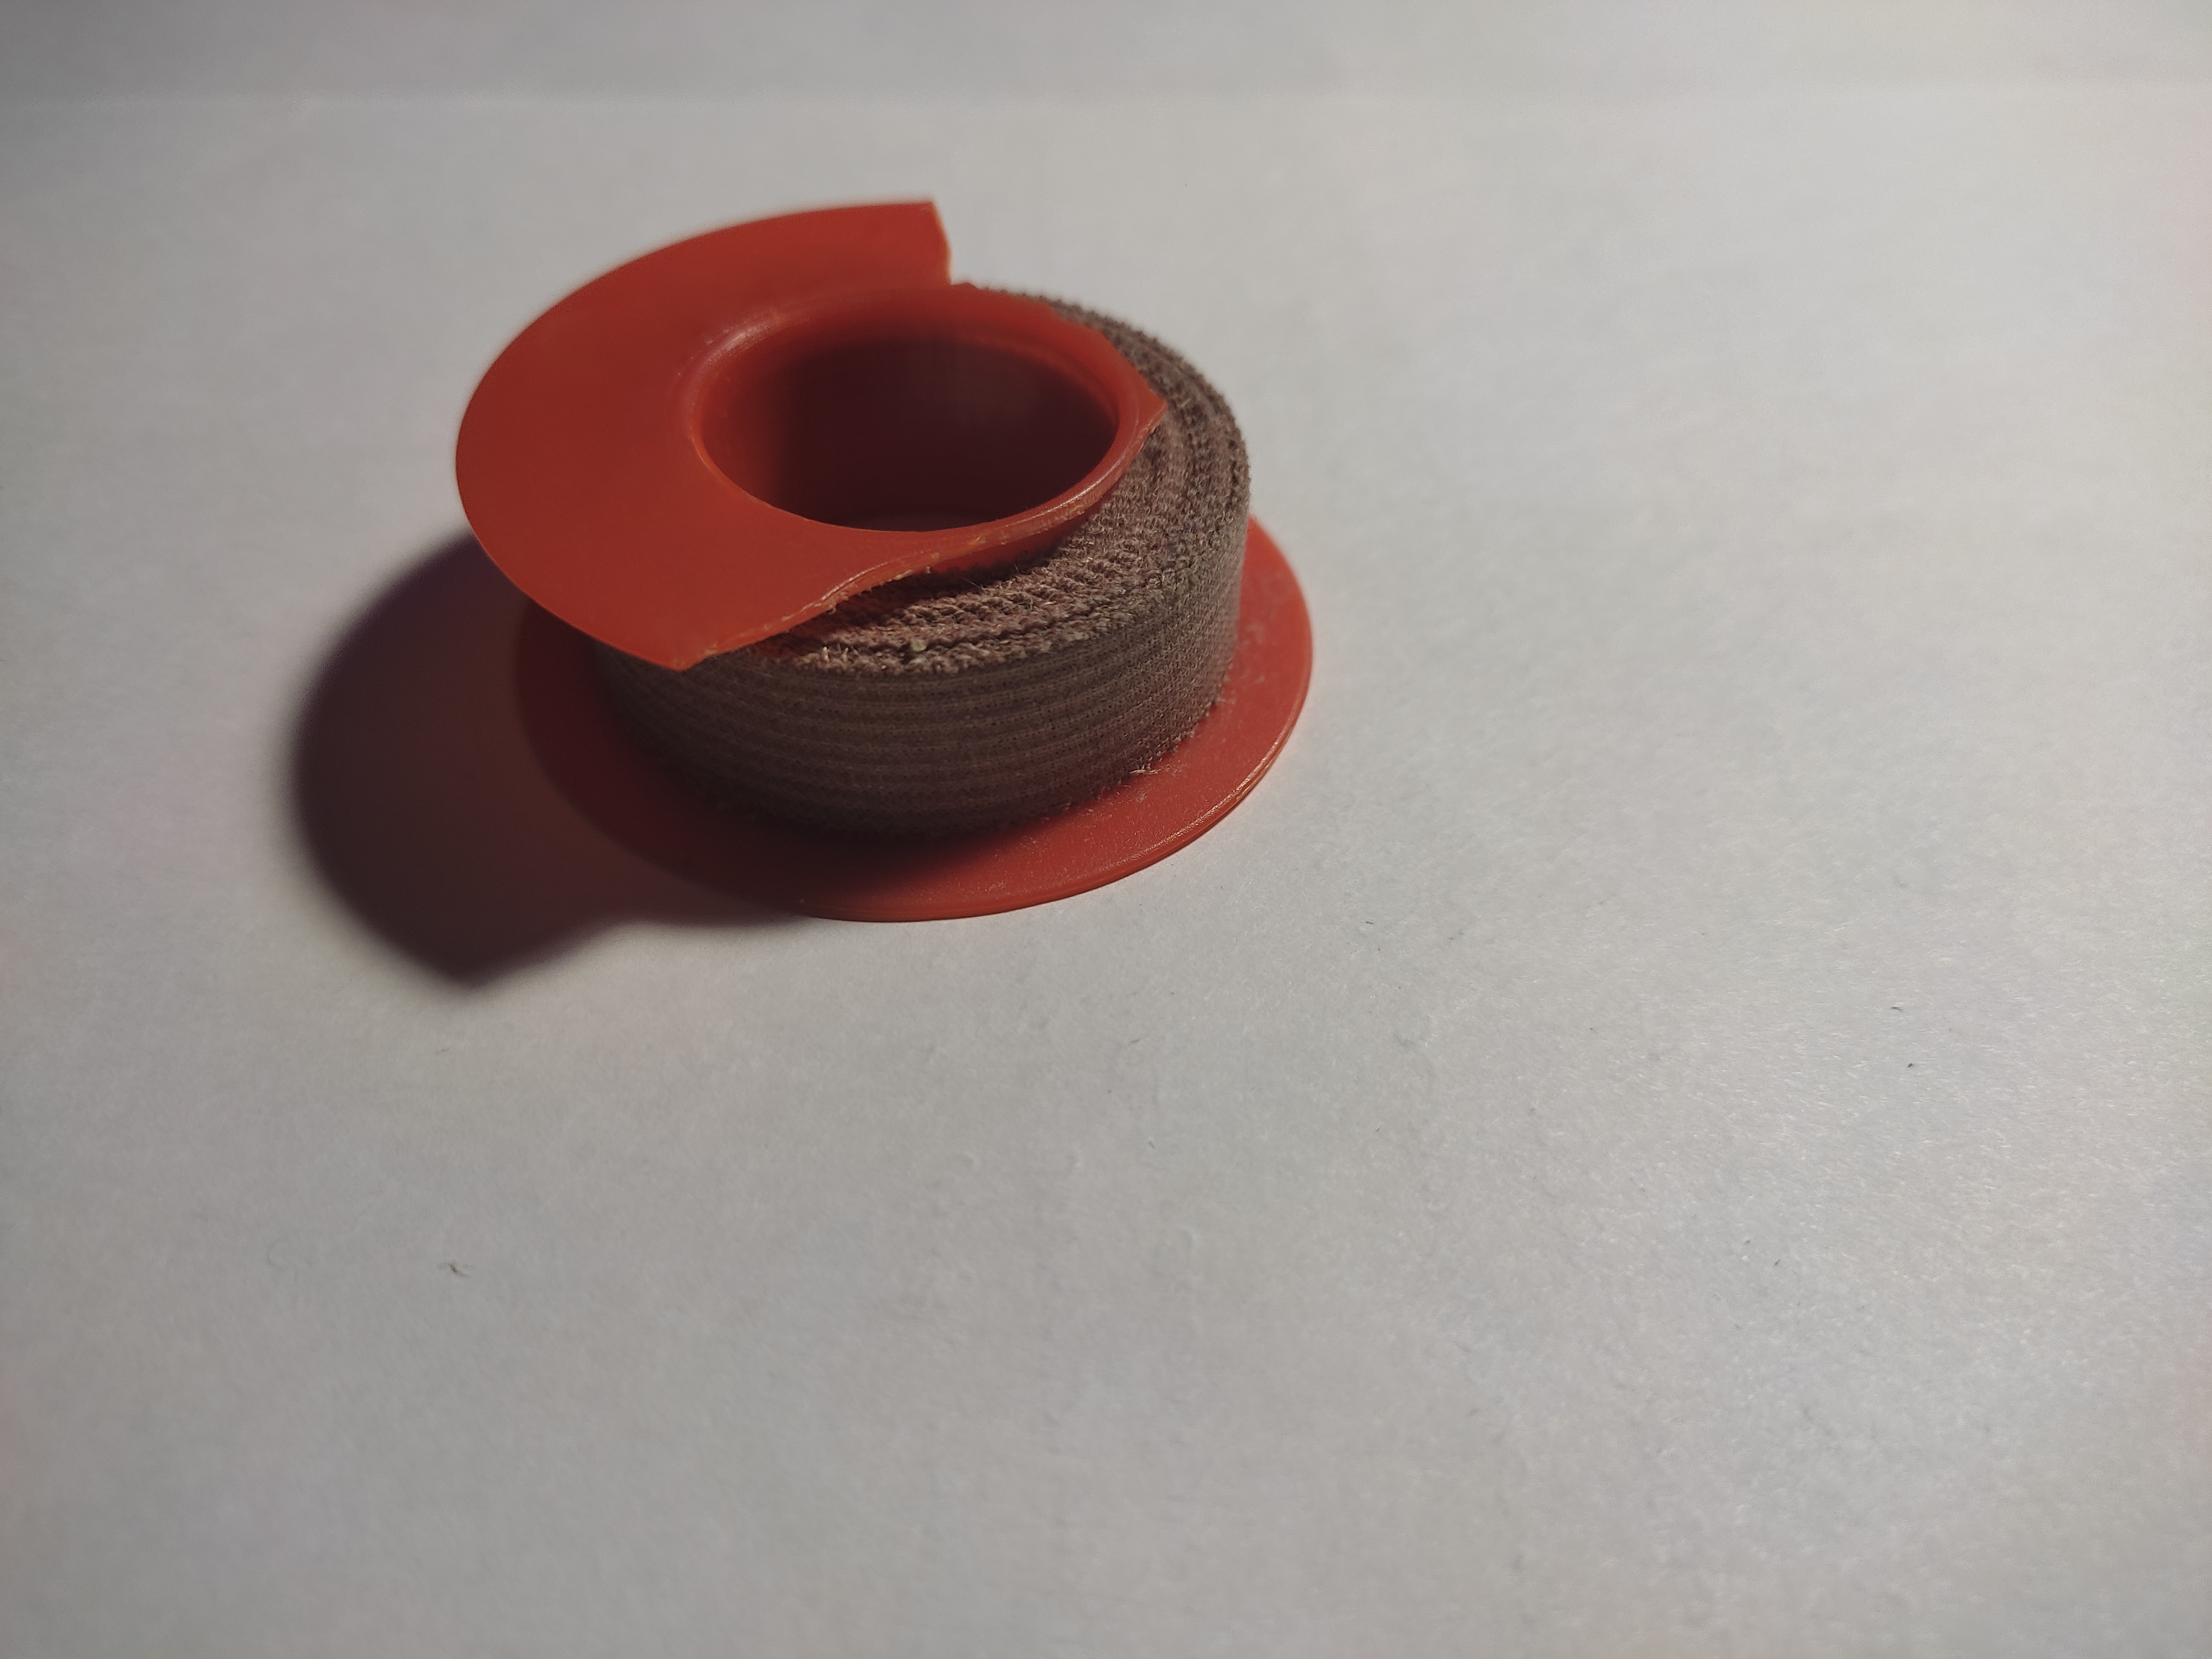
\includegraphics[width=0.7\linewidth]{катушка_от_сани.jpeg}
    \label{fig:i1}
}
\vskip 1cm
{\bf Свойства объекта, которые необходимо отразить}

Форма в виде катушки.

Объект состоит из двух частей: лейкопласторной ленты, пластикового каркаса. 

Цвет пластикового каркаса - красный.

Цвет лейкопластырной ленты - сиренево-коричневый.

Деффект на одной из граней катушки в виде отломанной части.




\section{Технология моделирования объектов}
\subsection{Технология создания модели объекта № 1}

\begin{enumerate}

\item Создание кривой вращения:

Добавление объекта "Кривая: 
Открыть меню<<Добавление объектов>> нажатием shift+A   $\to $  Curve  $\to $ Bezier.

На экране появится кривая, которую в дальнейшем нужно будет модифицировать:


\vskip 1cm
{
    \centering
    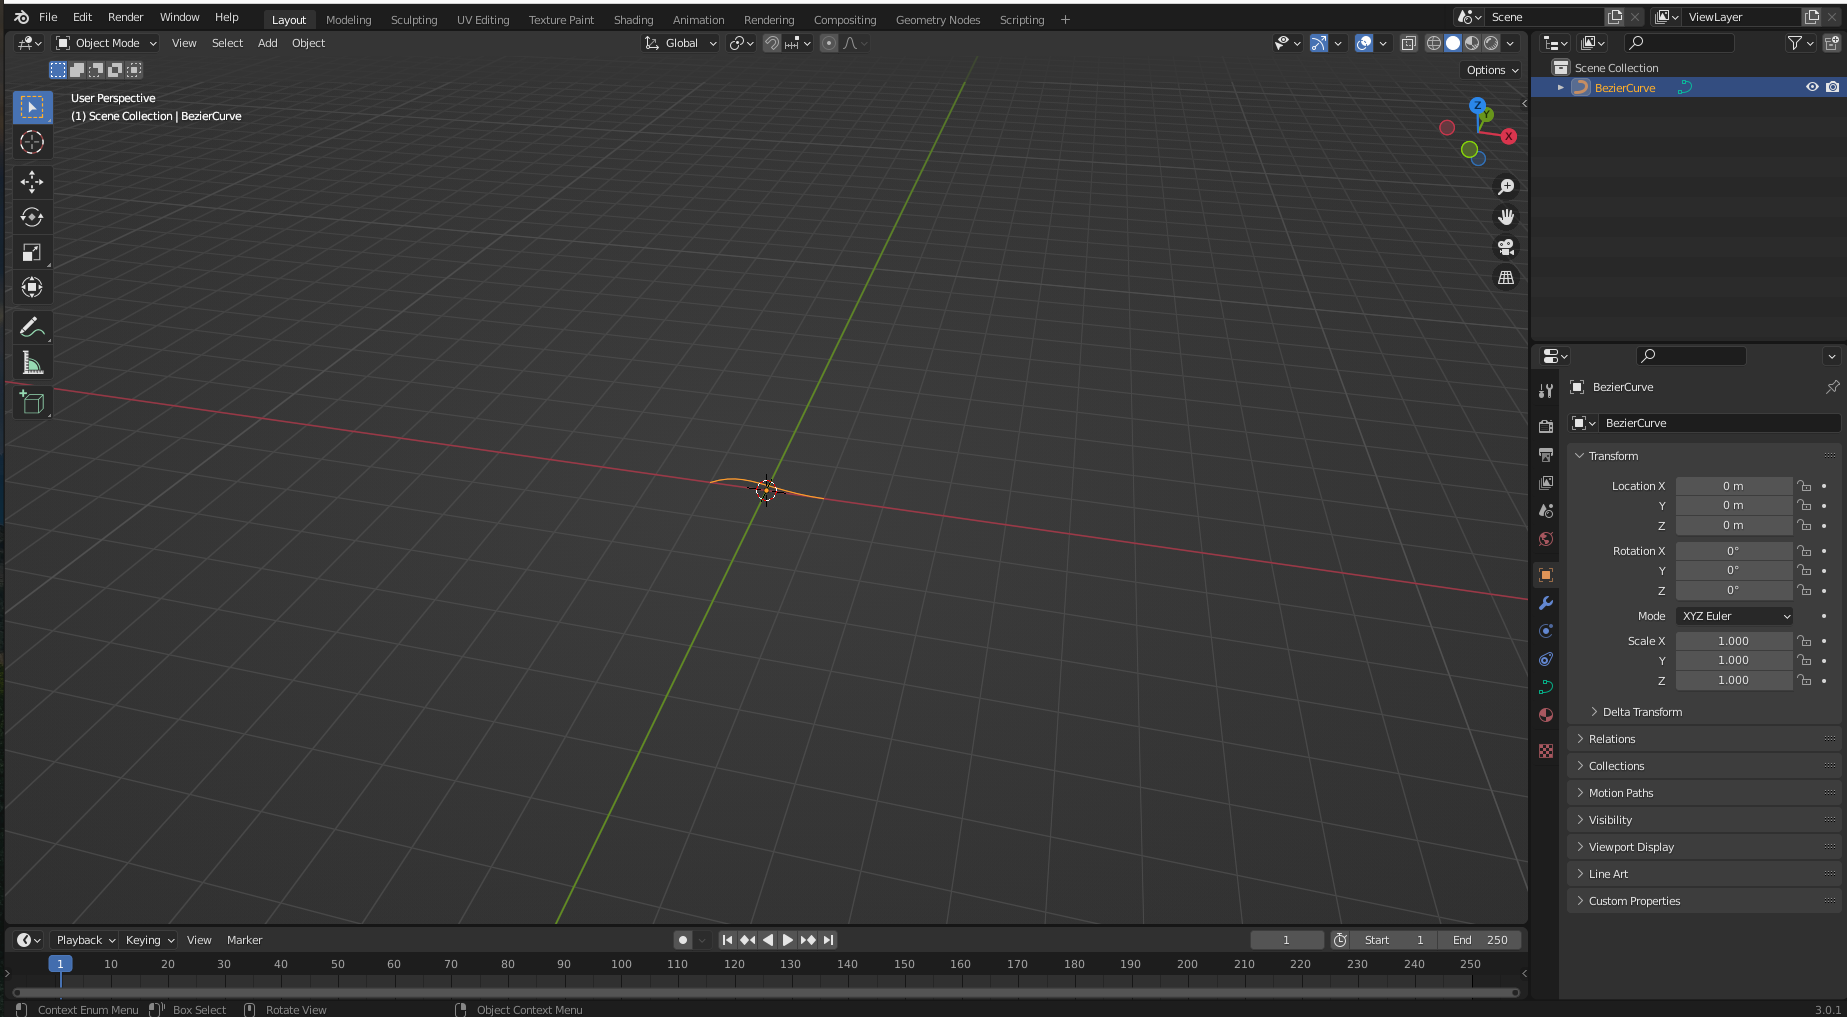
\includegraphics[width=1\linewidth]{кривая1.png}
    \label{fig:i1}
}
\vskip 1cm


\item Задание кривой необходимой формы:

Переходим в режим <<Edit mode>> нажатием табуляции  $\to $   переходим в инструмент <<Add points>>(зеленая иконка в правом нижнем углу)  $\to $ выделяем поочереди точки на кривой нажатием на неё $\to $ выставляем координаты каждой из точек в окне установки координат в правом углу экрана.

В итоге получим следующую форму ломаной.
\vskip 1cm
{
    \centering
    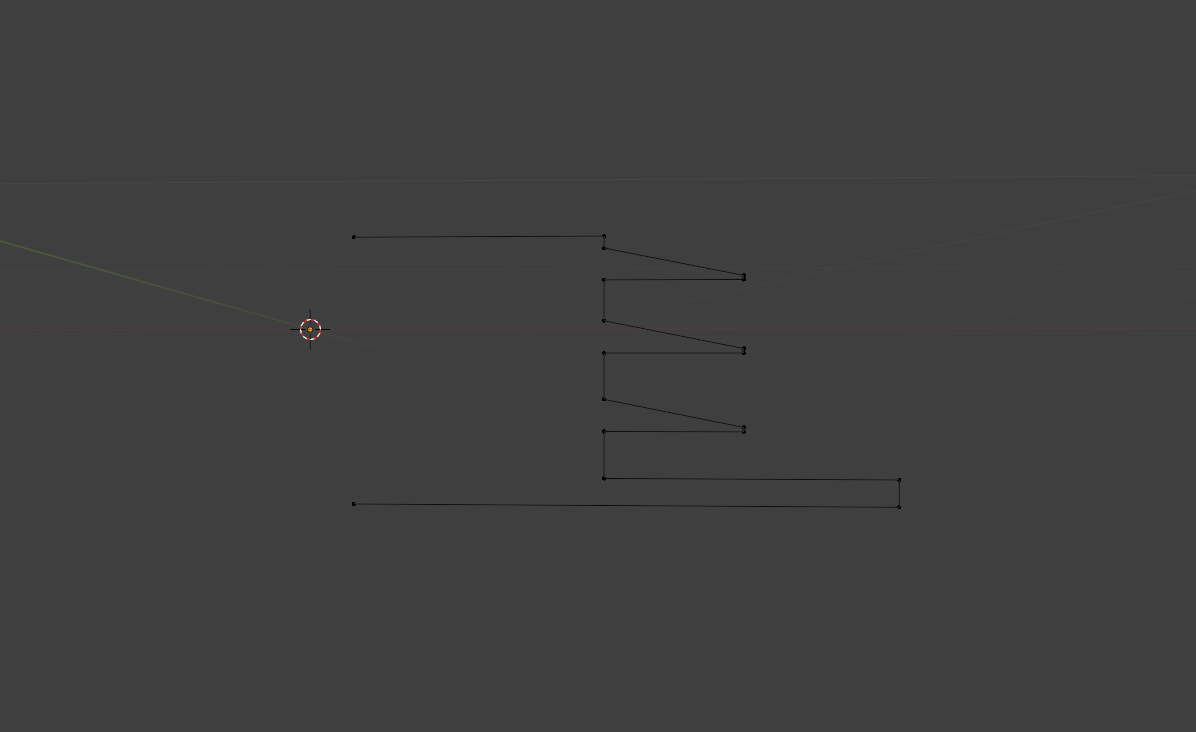
\includegraphics[width=1\linewidth]{форма1.png}
    \label{fig:i1}
}
\vskip 1cm


Ниже представленны координаты в миллиметрах для каждой из точкек и расстановка точек на ломаной.


Расстановка точек:
\vskip 1cm
{
    \centering
    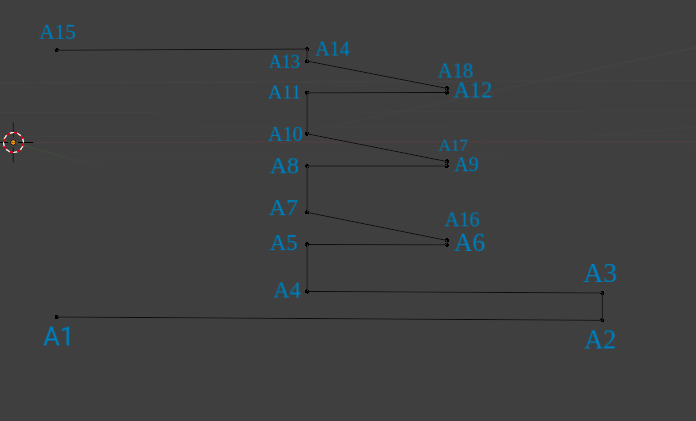
\includegraphics[width=1\linewidth]{кривая_с_точками.png}
    \label{fig:i1}
}
\vskip 1cm


Координаты точек:


A1=\{0,0,0\};

A2=\{32,0,0\};

A3=\{32,0,2\};

A4=\{15,0,2\};

A5=\{15,0,6\};

A6=\{22,0,6\};

A8=\{15,0,14\};

A9=\{22,0,14\};

A10=\{15,0,17\};

A11=\{15,0,21\};

A12=\{22,0,21\};

A13=\{15,0,24\};

A14=\{15,0,25\};

A15=\{0,0,25\};

A16=\{22,0,6.5\};

A17=\{22,0,14.5\};

A18=\{22,0,21.5\};






\item Примение модификатора <<Screw>> к кривой.

Перейти во вкладку <<Modifiers>> $\to $ нажать <<Add Modifier>>  $\to $ выбрать <<Screw>>  $\to $ изменить параметр <<Axis>> на <<Y>>(задаем ось вращения), <<angle>> - 360 $\to $  изменить <<Randor>> и <<Steps Viewport>> на 60(делаем модель более сглаженной) $\to $ нажимаем <<apply>>.



После этого на экране увидим следующее:

\vskip 1cm
{
    \centering
    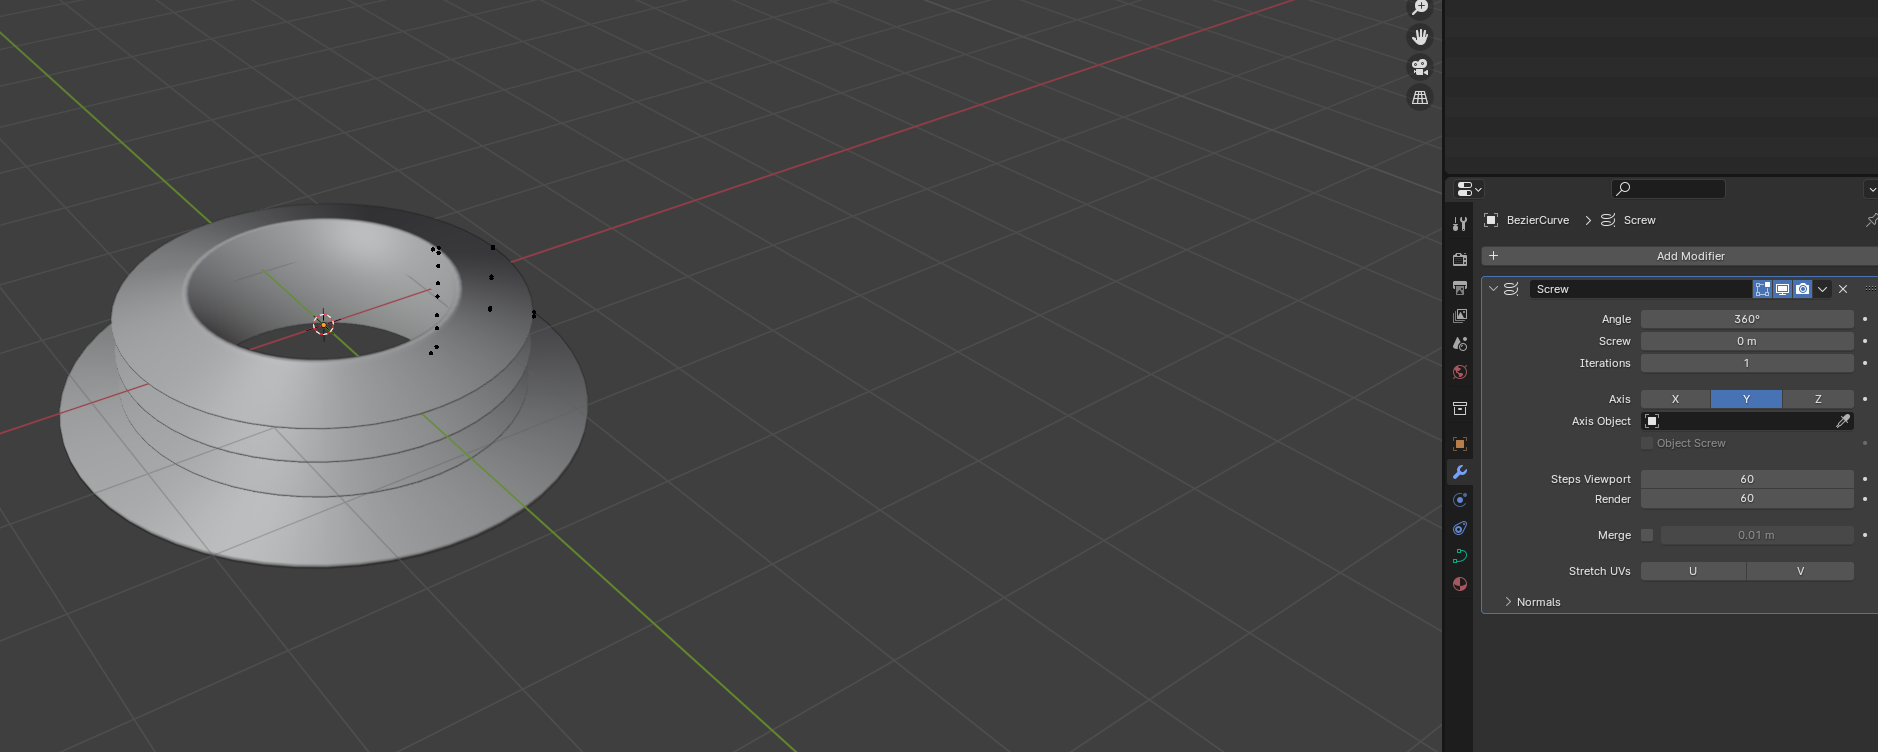
\includegraphics[width=1\linewidth]{форма2.png}
    \label{fig:i1}
}
\vskip 1cm

Затем нужно конвертировать объект в mesh( сетку из вершин и граней) для дальнейшего редактирования.

Нажать:<<Object>>$\to $<<convert>>$\to $<<mesh>>.


\item Модуляция дефекта в основании клапана.

Нажать Shift+пробел для открытия окна выбора инструментов $\to $ выбрать <<draw>>(рисование) $\to $ провести кривую нужной формы для выреза дефекта. 

Вид полученной кривой:

\vskip 1cm
{
    \centering
    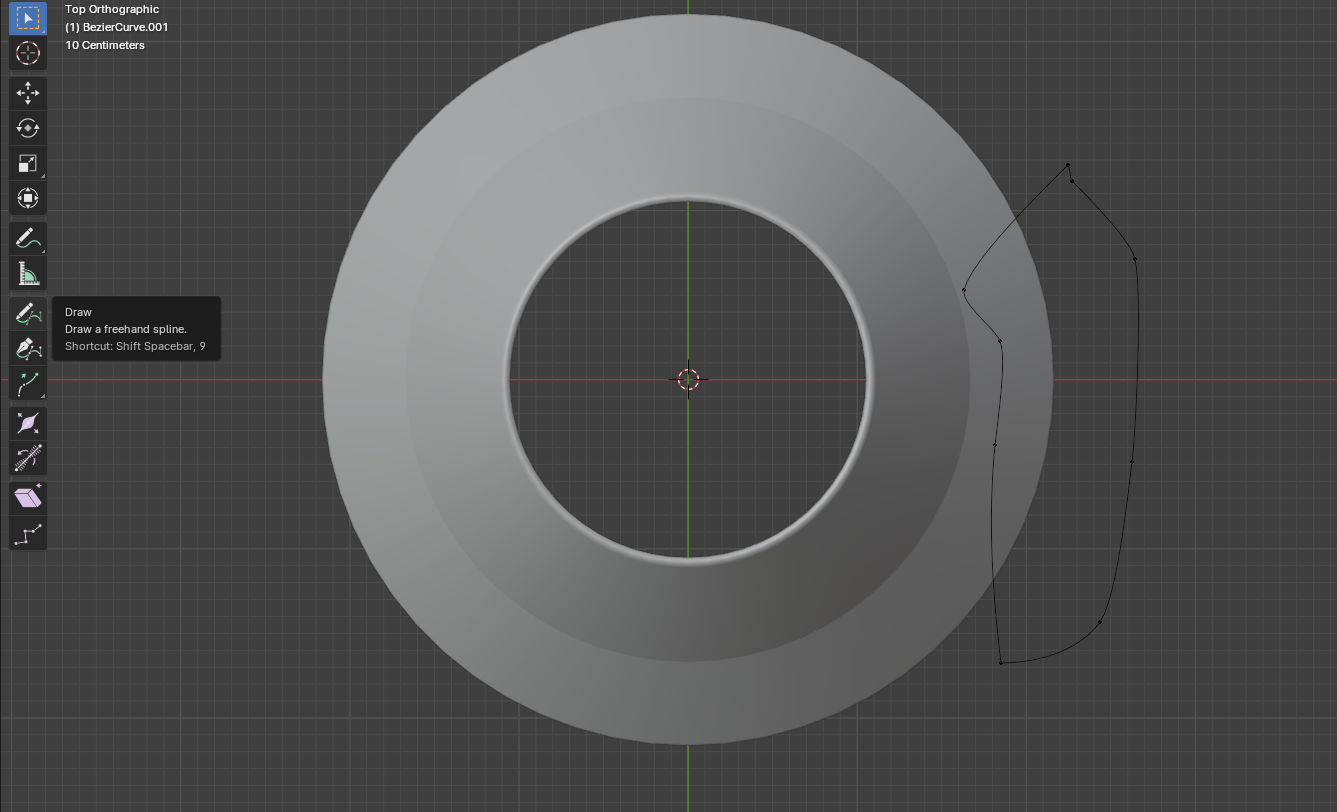
\includegraphics[width=1\linewidth]{кривая_дефекта.png}
    \label{fig:i1}
}
\vskip 1cm


После этого нужно нажать правой кнопкой мыши на объект и выбрать в сплывающем окне <<New face from edges>> для получения плоскости по кривой.

\item Создание объемного объекта для моделирования дефекта в основании клапана.

Перейти в инструмент <<Extrude>>  $\to $ выделить плоскость $\to $ нажать правой кнопкой мыши$\to $ выбрать поле <<Extrude region and move>> $\to $ изменить значение по оси Z на 5 mm.


Получим следующий вид модели:

\vskip 1cm
{
    \centering
    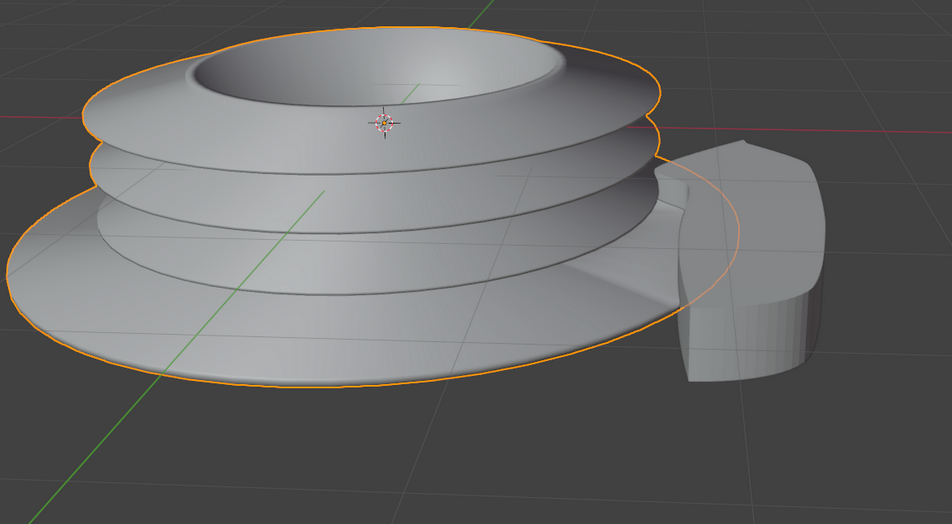
\includegraphics[width=1\linewidth]{форма_с_об_диф.png}
    \label{fig:i1}
}
\vskip 1cm
	
\item Вырез области для получения дефекта в основании модели.

Выделить основную форму $\to $ Выбрать <<Modifier properties>> на панели инструментов $\to $ в выподающем окне <<Add modifier>>  выбрать модификатор <<Boolean>> $\to $ указать параметр <<Difference>> в панели параметров модификатора $\to $ выделить вторую модель для применения модификатора $\to $ нажать <<apply>>.

На экране получим следущий вид модели:

\vskip 1cm
{
    \centering
    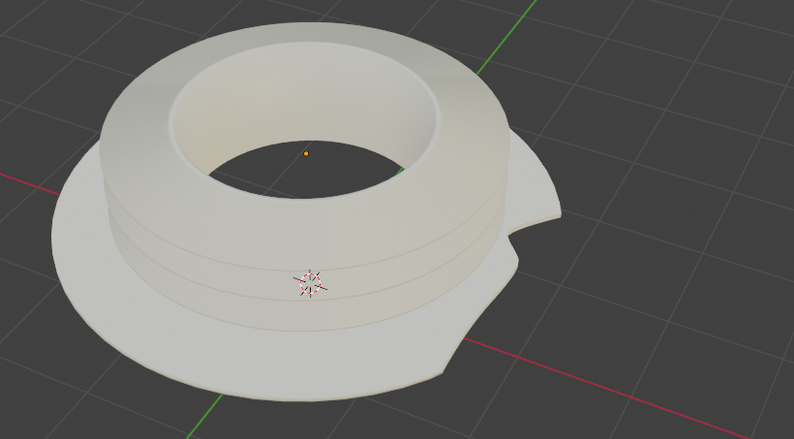
\includegraphics[width=1\linewidth]{final1.png}
    \label{fig:i1}
}
\vskip 1cm





\item Задаем цвет и параметры материала модели:

Переходим в <<Material properties>> на панели инструментов $\to $ во вкладке <<surface>> указываем следующие параметры:

Base color:  устанавливаем цвет наиболее похожий на реальный цвет модели.

Metallic: 0  -  значение, обозначающее металлический блеск поверхности (0 -отсутсвие блеска)

Roughness: 0.5  - значение, обозначающее коэфицент шероховатости поверхности

IOR:  1.450 - значение, обозначающее приломление света для материала. 

alpha: 1.000 - значение, обозначающее  прозрачность материала.


Нажимаем f12 и дожидаемся окончания рендеринга
\end{enumerate}


{\bf Результат работы:}


Ниже представлен итоговый результат моделирования объекта.


\vskip 1cm
{
    \centering
    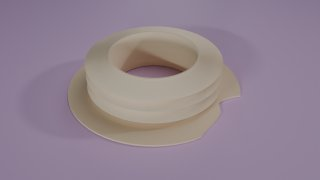
\includegraphics[width=1\linewidth]{клапан_финал.png}
    \label{fig:i1}
}
\vskip 1cm

    
    
    
    
    
    
    
    
    
    
    
    
    
    
    
\subsection{Технология создания модели объекта № 2}


\begin{enumerate}

\item Создание линии, повторяющей форму ручки ключа:


Открыть меню<<Добавление объектов>> нажатием shift+A   $\to $  Curve  $\to $ Bezier.

На экране появится кривая, которую в дальнейшем нужно будет модифицировать:


\vskip 1cm
{
    \centering
    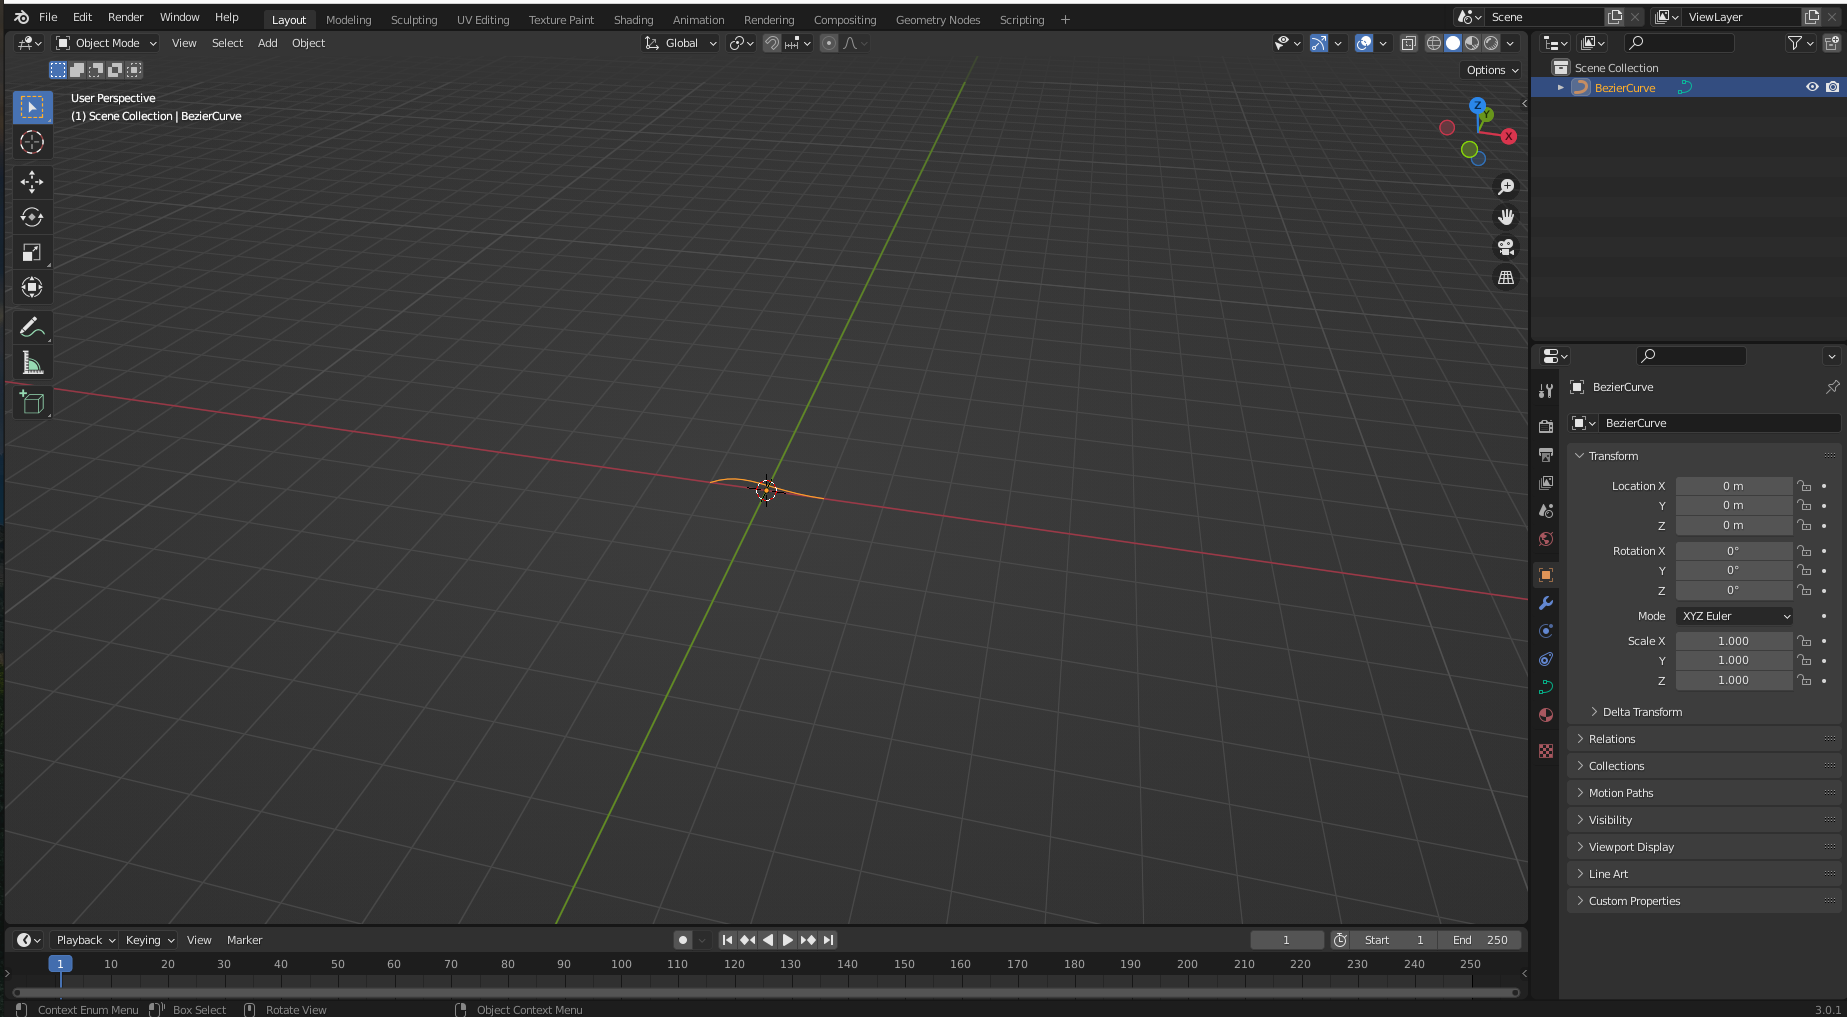
\includegraphics[width=1\linewidth]{кривая1.png}
    \label{fig:i1}
}
\vskip 1cm


Задание необходимой формы для кривой:

Переходим в режим <<Edit mode>> нажатием табуляции  $\to $   переходим в инструмент <<Add points>>(зеленая иконка в правом нижнем углу)  $\to $ выделяем точки по очереди и вручную выставляем их в соответствии с формой ручки ключа.

Получим следующий вид ломаной:
\vskip 1cm
{
    \centering
    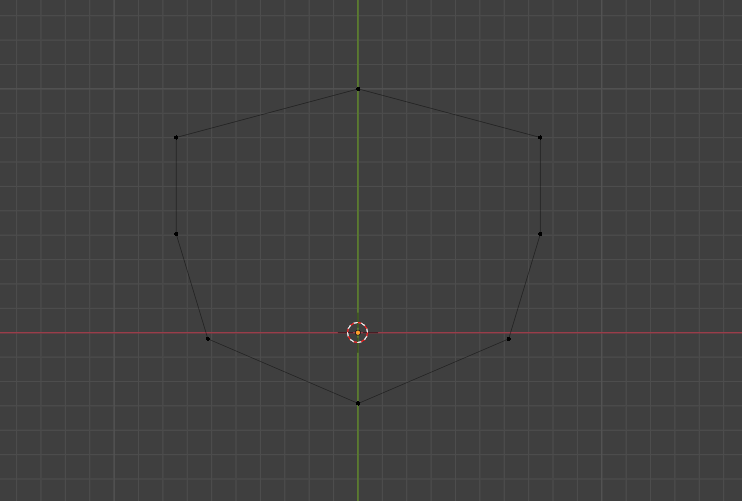
\includegraphics[width=0.7\linewidth]{3кривая1.png}
    \label{fig:i1}
}
\vskip 1cm

\item Создание объёмной формы ручки ключа:

Выделить полученную линию $\to $ кликнуть правой кнопкой мыши $\to $ в выпадающем меню выбрать <<New face from edges>>  $\to $ выбрать инструмент <<Extrude>> на левой панели инструментов  $\to $ в нижнем правом углу в выподающем окне <<Extrude region and move>> указать значение 1 mm по оси Z.

Получим следующий вид модели:
\vskip 1cm
{
    \centering
    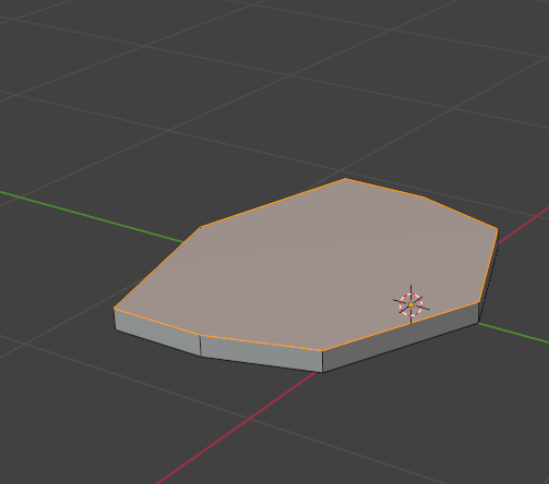
\includegraphics[width=0.7\linewidth]{3r1.png}
    \label{fig:i1}
}
\vskip 1cm

\item Снятие фаски (Сглаживание углов).

Для получения формы схожей с  реальным объектом, необходимо произвести снятие фаски. 

Снятие фаски для вертикальных граней:

Для перехода в инструмент снятия фаски нажать CTRL+B  $\to $ выделить вертикальные грани объекта  $\to $  в левой части экрана появится окно с параметрами снятия фаски. 

В окне указать:

<<Weight>>: 2mm

<<Segments>>: 3

Остальные параметры оставить по умолчанию.

Получим следующий вид модели:

\vskip 1cm
{
    \centering
    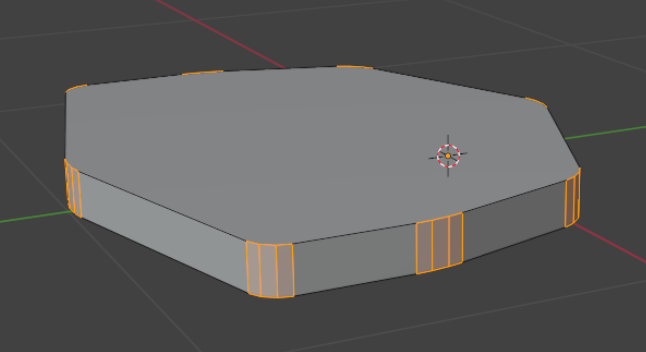
\includegraphics[width=0.7\linewidth]{3вертф.png}
    \label{fig:i1}
}
\vskip 1cm

Снятие фаски для горизонтальных граней:

Для перехода в инструмент снятия фаски нажать CTRL+B  $\to $ выделить горизонтальные грани объекта.

В окне параметров указать:

<<Weight>>: 1mm

<<Segments>>: 3

Остальные параметры оставить по умолчанию.

Получим следующий вид модели:

\vskip 1cm
{
    \centering
    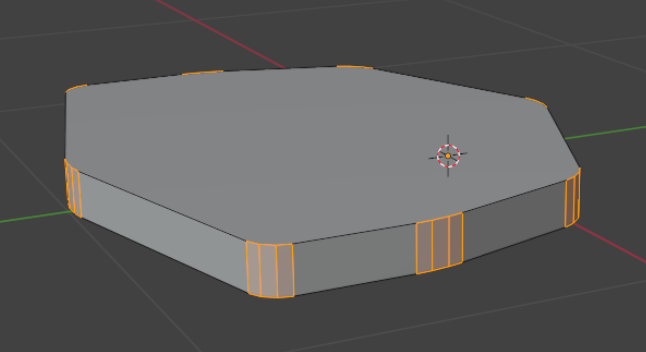
\includegraphics[width=0.7\linewidth]{3вертф.png}
    \label{fig:i1}
}
\vskip 1cm




\item Моделирование основы ключа циллиндрической формы.
Чтобы создать форму циллиндра нужно:

Нажать shift+A  для открытия окна добавления форм $\to $ выбрать <<mesh>> $\to $ выбрать <<Cylinder>>.

Получим следующий объект:

\vskip 1cm
{
    \centering
    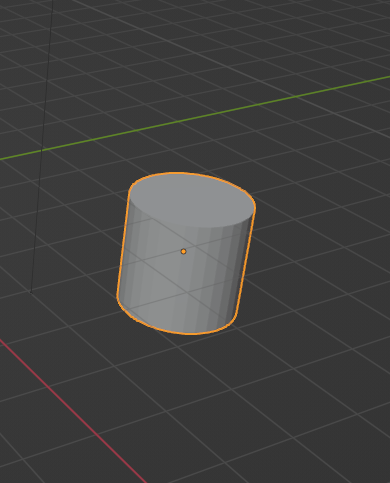
\includegraphics[width=0.7\linewidth]{3cyl1.png}
    \label{fig:i1}
}
\vskip 1cm

Теперь укажем необходимый радиус и длинну циллиндра в правой нижней части экрана.

В поле <<Depth>> установим 65 mm.

В поле <<Radius>> установим 2 mm.

Затем с помощью вращения(нажатие ctrl+R) и перемещения (нажатие ctrl+G)   полученный циллиндр выставляется в нужное место, смежно с ручкой ключа.

\vskip 1cm
{
    \centering
    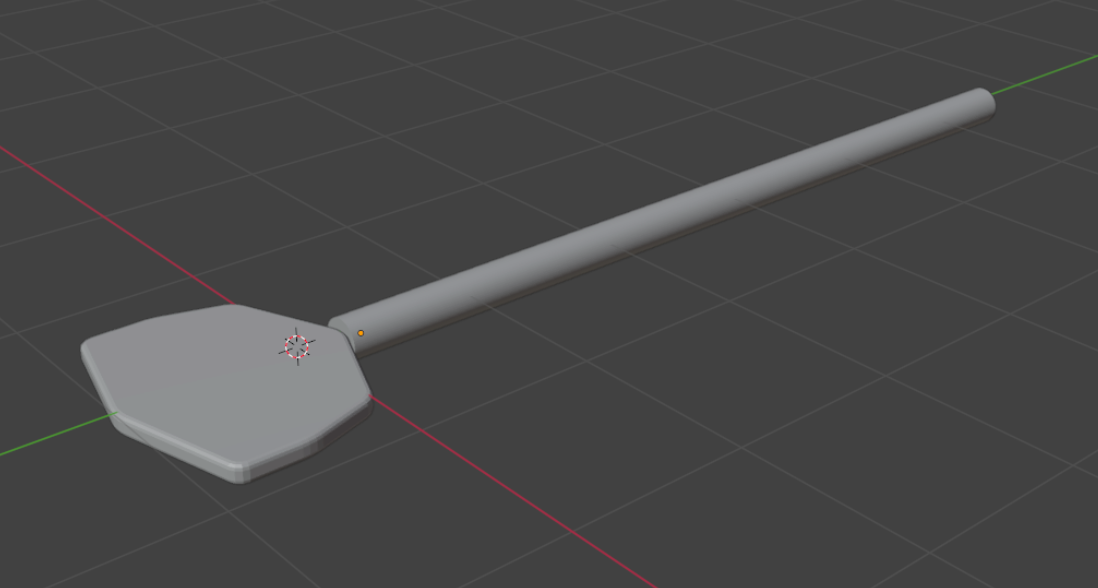
\includegraphics[width=1\linewidth]{cyl2.png}
    \label{fig:i1}
}
\vskip 1cm

После этого нужно применить сглаживание углов к каждому из концов циллиндра. Для этого:

Выделяем каждое из оснований $\to $ нажимаем ctrl+B  $\to $ указываем параметры в сплывающем окне в нижнем левом углу:

width: 2mm
Segments: 10

После сглаживания получим:

\vskip 1cm
{
    \centering
    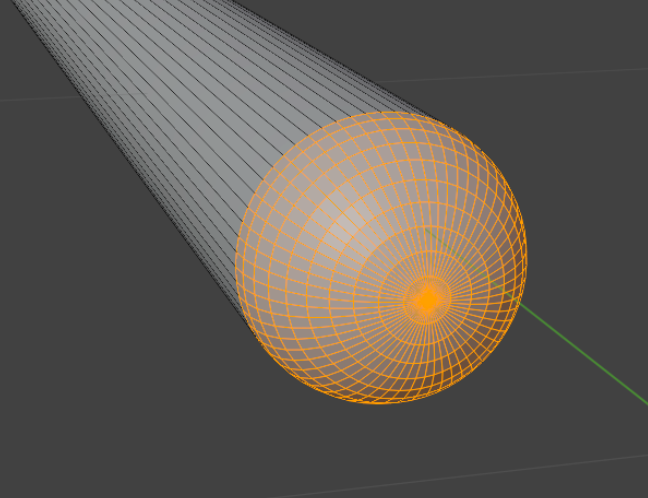
\includegraphics[width=0.8\linewidth]{3cyl3.png}
    \label{fig:i1}
}
\vskip 1cm


\item Создание отверстия на ручке ключа.

Создаем новый циллиндр с помощью:

Нажать shift+A  для открытия окна добавления форм $\to $ выбрать <<mesh>> $\to $ выбрать <<Cylinder>>.

Устанаваем Radius: 2mm, Depth: 6mm (в данном случае длина циллиндра нам не важна, можем установить любое значение болшее 2mm, ширины ручки ключа).

 С помощью вращения(нажатие ctrl+R) и перемещения (нажатие ctrl+G)   полученный циллиндр нужно выставить перпендикулярно плоскости ручки ключа в то место, где распологается отверстие в реальном объекте. Циллиндр нужно установить так, чтобы он проходил через ручку ключа насквозь.
 
Нужно добиться следующего расположения объектов:

\vskip 1cm
{
    \centering
    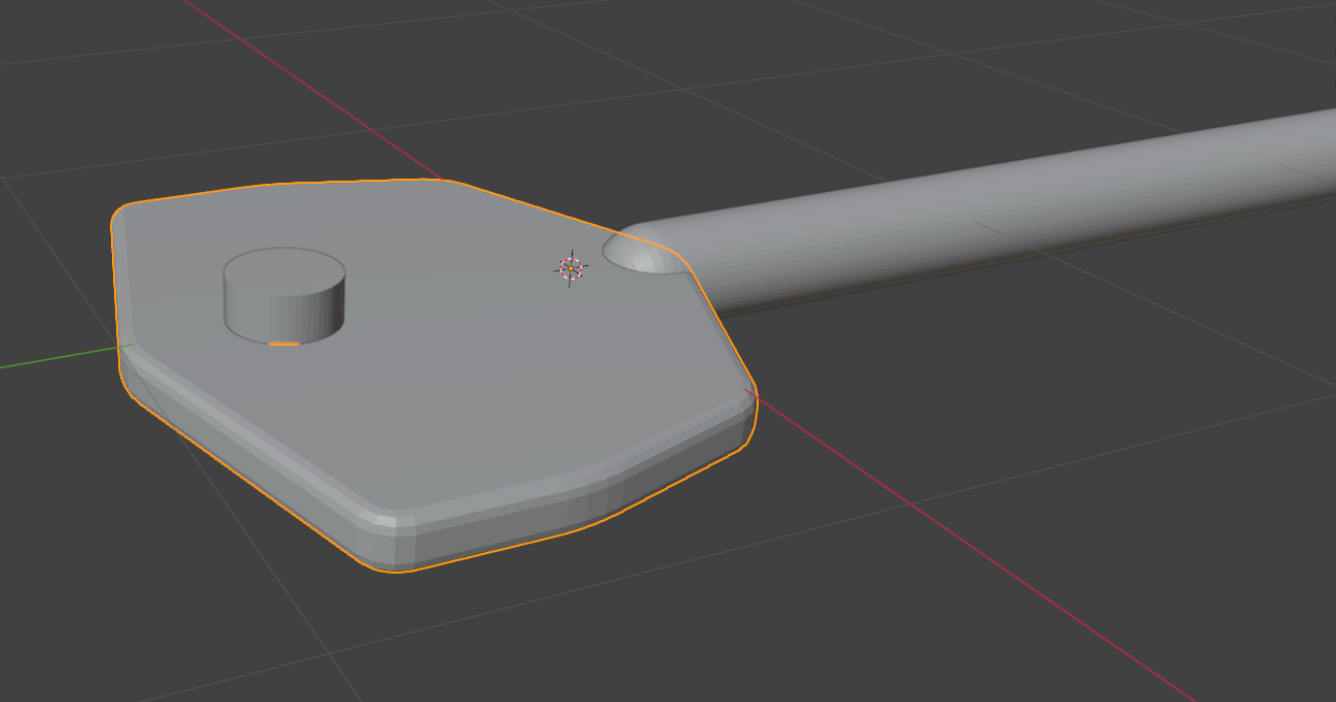
\includegraphics[width=0.8\linewidth]{3cyl4.png}
    \label{fig:i1}
}
\vskip 1cm
 

После этого нужно применить модификатор Boolean с параметром Difference к форме ручки ключа. Для этого:


Выделить форму ручки ключа $\to $ Выбрать <<Modifier properties>> на панели инструментов $\to $ в выподающем окне <<Add modifier>>  выбрать модификатор <<Boolean>> $\to $ указать параметр <<Difference>> на панели параметров модификатора $\to $ выделить полученный циллиндр $\to $ нажать <<apply>>.

В результате применения получим:

\vskip 1cm
{
    \centering
    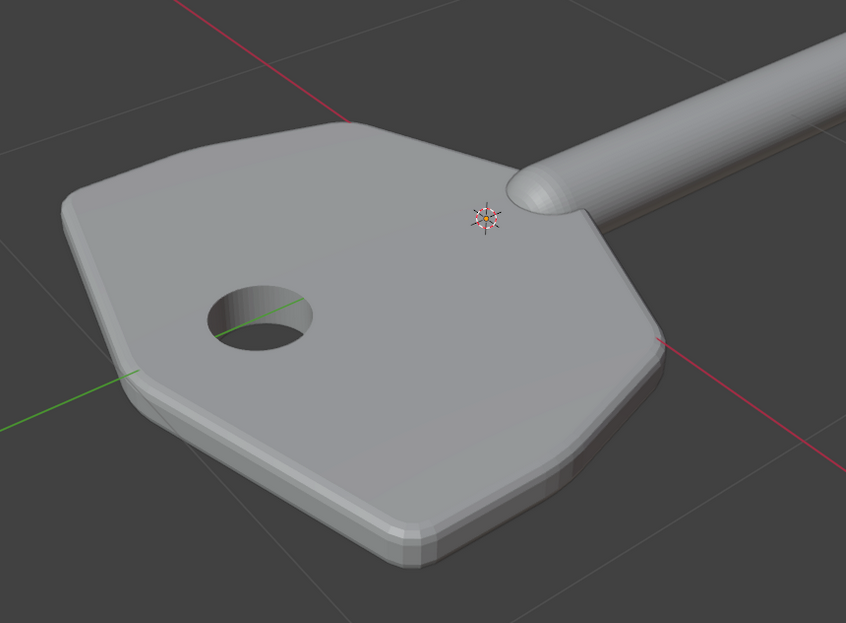
\includegraphics[width=0.8\linewidth]{3дыра.png}
    \label{fig:i1}
}
\vskip 1cm





\item Создание рабочей части ключа.

Нажать shift+A  для открытия окна добавления форм $\to $  <<mesh>> $\to $ выбрать <<plane>>(плоскость) $\to $  на экране появится плоскость размера по умолчанию, размер не меняем.

Далее нужно разбить плоскость по сетке для задания отверстий в рабочей части ключа в соответсвии с реальным видом объекта.

Для этого:  переходим в режим редактирования, нажав клавишу табуляции $\to $ выбираем инструмент <<Subdivide>> из панели инструментов в левой части экрана $\to $ В окне настройки инструмента Subdivide устнавливаем количество разрезов <<Number of cuts>> по ширине и по высоте.

По ширине: 4

По высоте: 2



В итоге получим следующий вид сетки:
\vskip 1cm
{
    \centering
    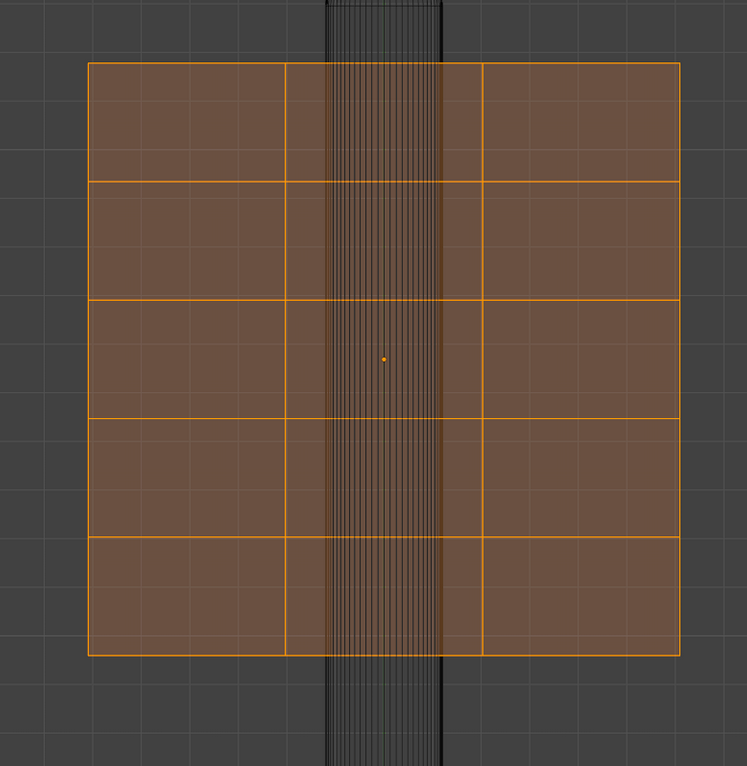
\includegraphics[width=0.8\linewidth]{3сетка.png}
    \label{fig:i1}
}
\vskip 1cm


Затем нужно удалить из сетки области, обозначающие вырезы в рабочей части ключа.
Для этого выбираем <<Edge Select>> и последовательно нажимаем необходимые для удаления области.

После выделения нажимаем на клавишу <<Delete>>

Получим следующий вид сетки:

\vskip 1cm
{
    \centering
    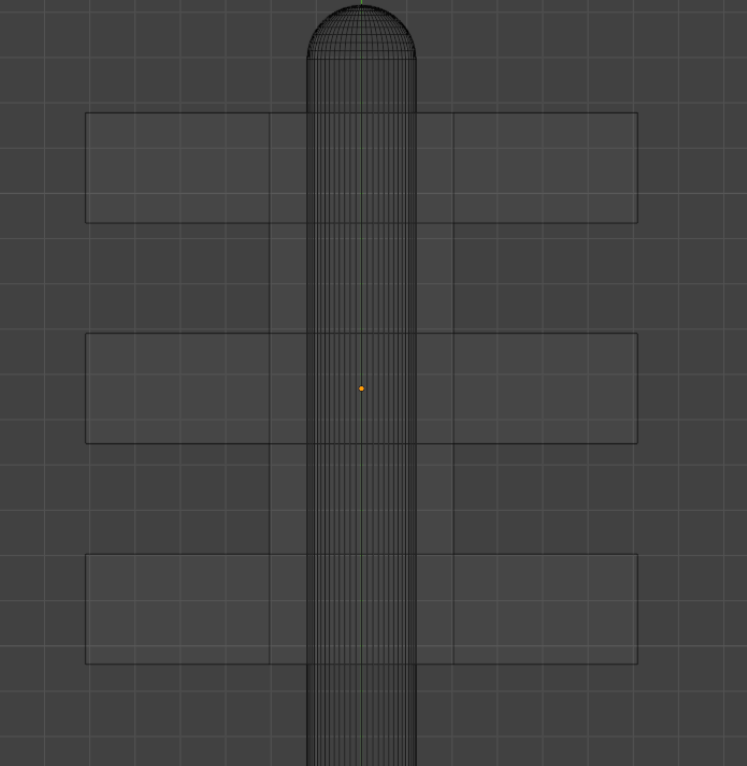
\includegraphics[width=0.8\linewidth]{3сетка2.png}
    \label{fig:i1}
}
\vskip 1cm

Путем последовательного выделения нужных граней и перемещения нажатием (ctrl+G) и движением мыши получим следующий вид сетки:


\vskip 1cm
{
    \centering
    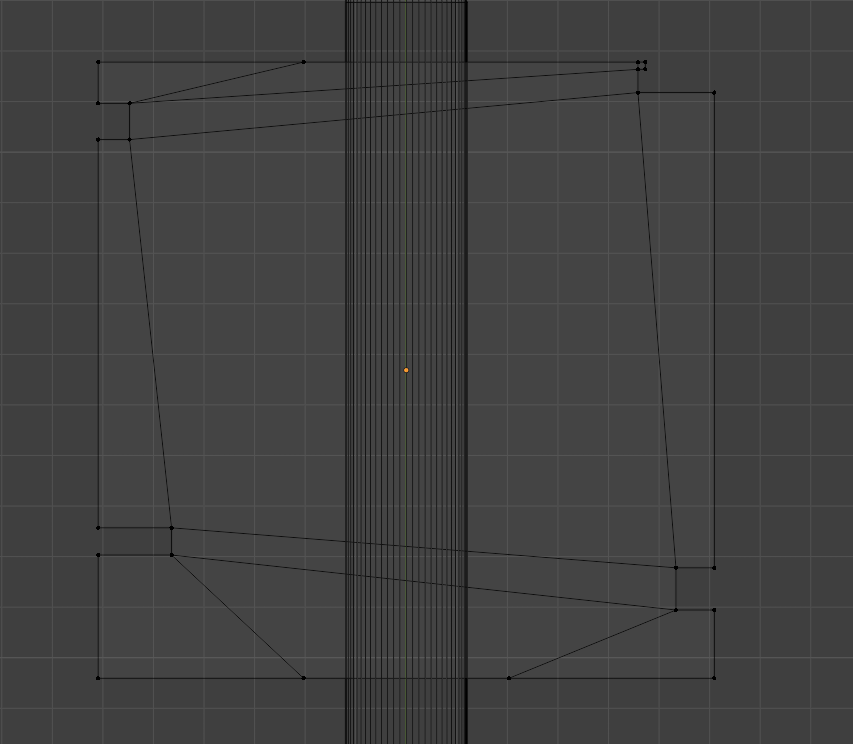
\includegraphics[width=0.8\linewidth]{3сет3.png}
    \label{fig:i1}
}
\vskip 1cm

После этого создаем объемный объект с помощью 
экструдирования плоскости. Для этого:


 Выбрать инструмент <<Extrude>> на левой панели инструментов  $\to $ в нижнем правом углу в выподающем окне <<Extrude region and move>> указать значение 2 mm по оси Z.
 



После создания рабочей части ключа ее нужно совместить с основной частью.

С помощью вращения(нажатие ctrl+R) и перемещения (нажатие ctrl+G)   полученную форму перемещаем в место расположения, как на реальной модели.

Совмещенные основная и рабочая части ключа:

\vskip 1cm
{
    \centering
    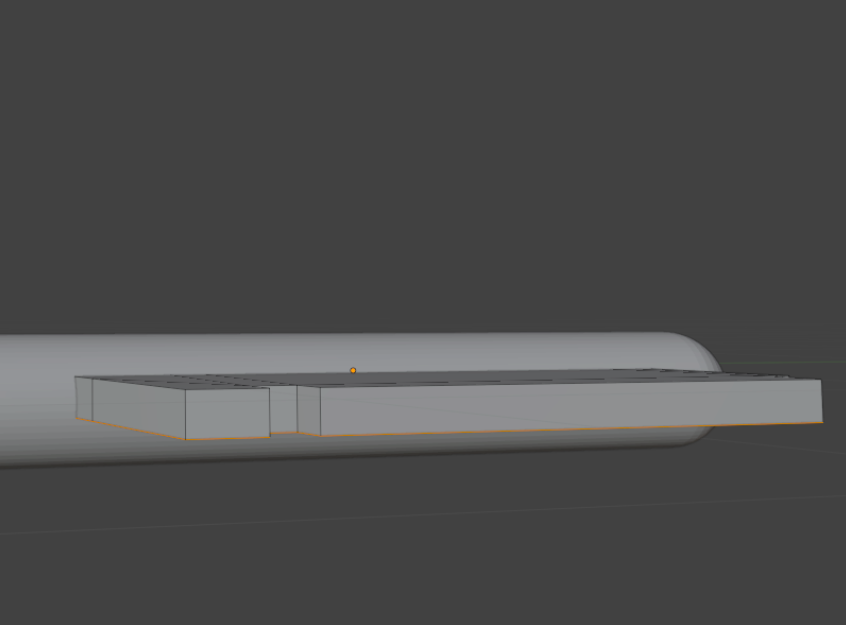
\includegraphics[width=0.8\linewidth]{3сов.png}
    \label{fig:i1}
}
\vskip 1cm



\item Выбор цвета и материала ключа:

Переходим в <<Material properties>> на панели инструментов $\to $ во вкладку <<surface>> $\to $ <<Base color>> $\to $ в поле <<Set color>> выберем из представленных наиболее похожий цвет на оригинальный цвет объекта.

Кроме этого выделим:

Metallic: 0.96  -  обозначает металлический блеск поверхности

Roughness: 0.4  - обозначает значение шероховатости поверхности

IOR:  1.450 - значение обозначающее приломление света для материала. 

alpha: 1.000 - обозначает прозрачность материала.

Полученная модель:

\vskip 1cm
{
    \centering
    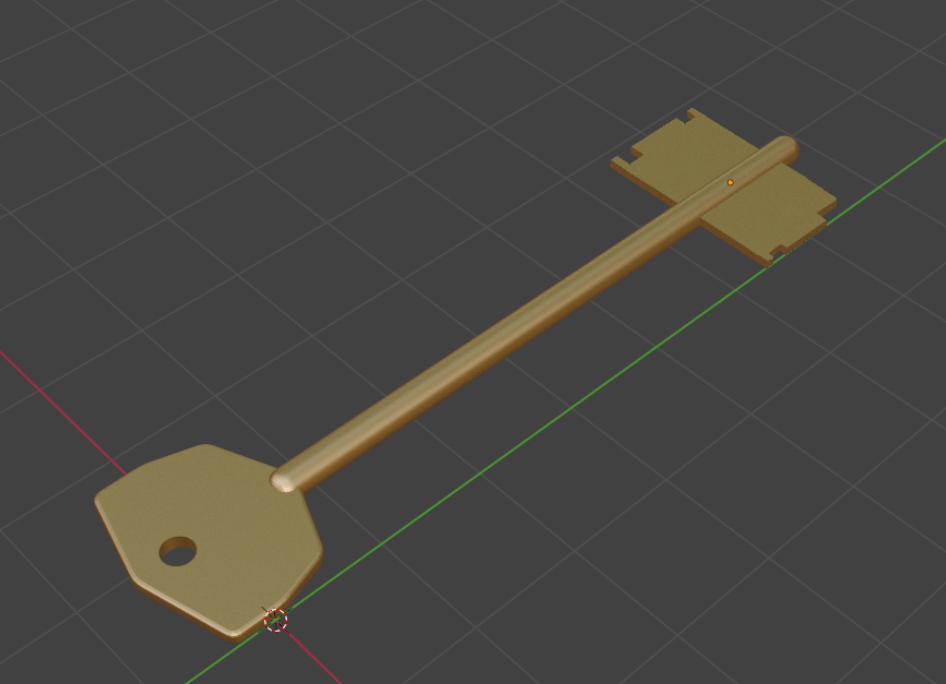
\includegraphics[width=0.8\linewidth]{3final0.png}
    \label{fig:i1}
}
\vskip 1cm




\item Нажимаем f12 и дожидаемся завершения рендеринга.



Итоговая версия модели:


\vskip 1cm
{
    \centering
    \includegraphics[width=0.8\linewidth]{ключ_рендер.png}
    \label{fig:i1}
}
\vskip 1cm



\end{enumerate} 
    
    
    
    
    
    
    
    
    
    
    
    
    
    
    
    
    
    
    
    
    




\subsection{Технология создания модели объекта № 3}


\begin{enumerate}
\item Cоздание кривой вращения:

Добавление объекта "Кривая: 
Открыть меню<<Добавление объектов>> нажатием shift+A   $\to $  Curve  $\to $ Bezier.

На экране появится кривая, которую в дальнейшем нужно будет модифицировать:


\vskip 1cm
{
    \centering
    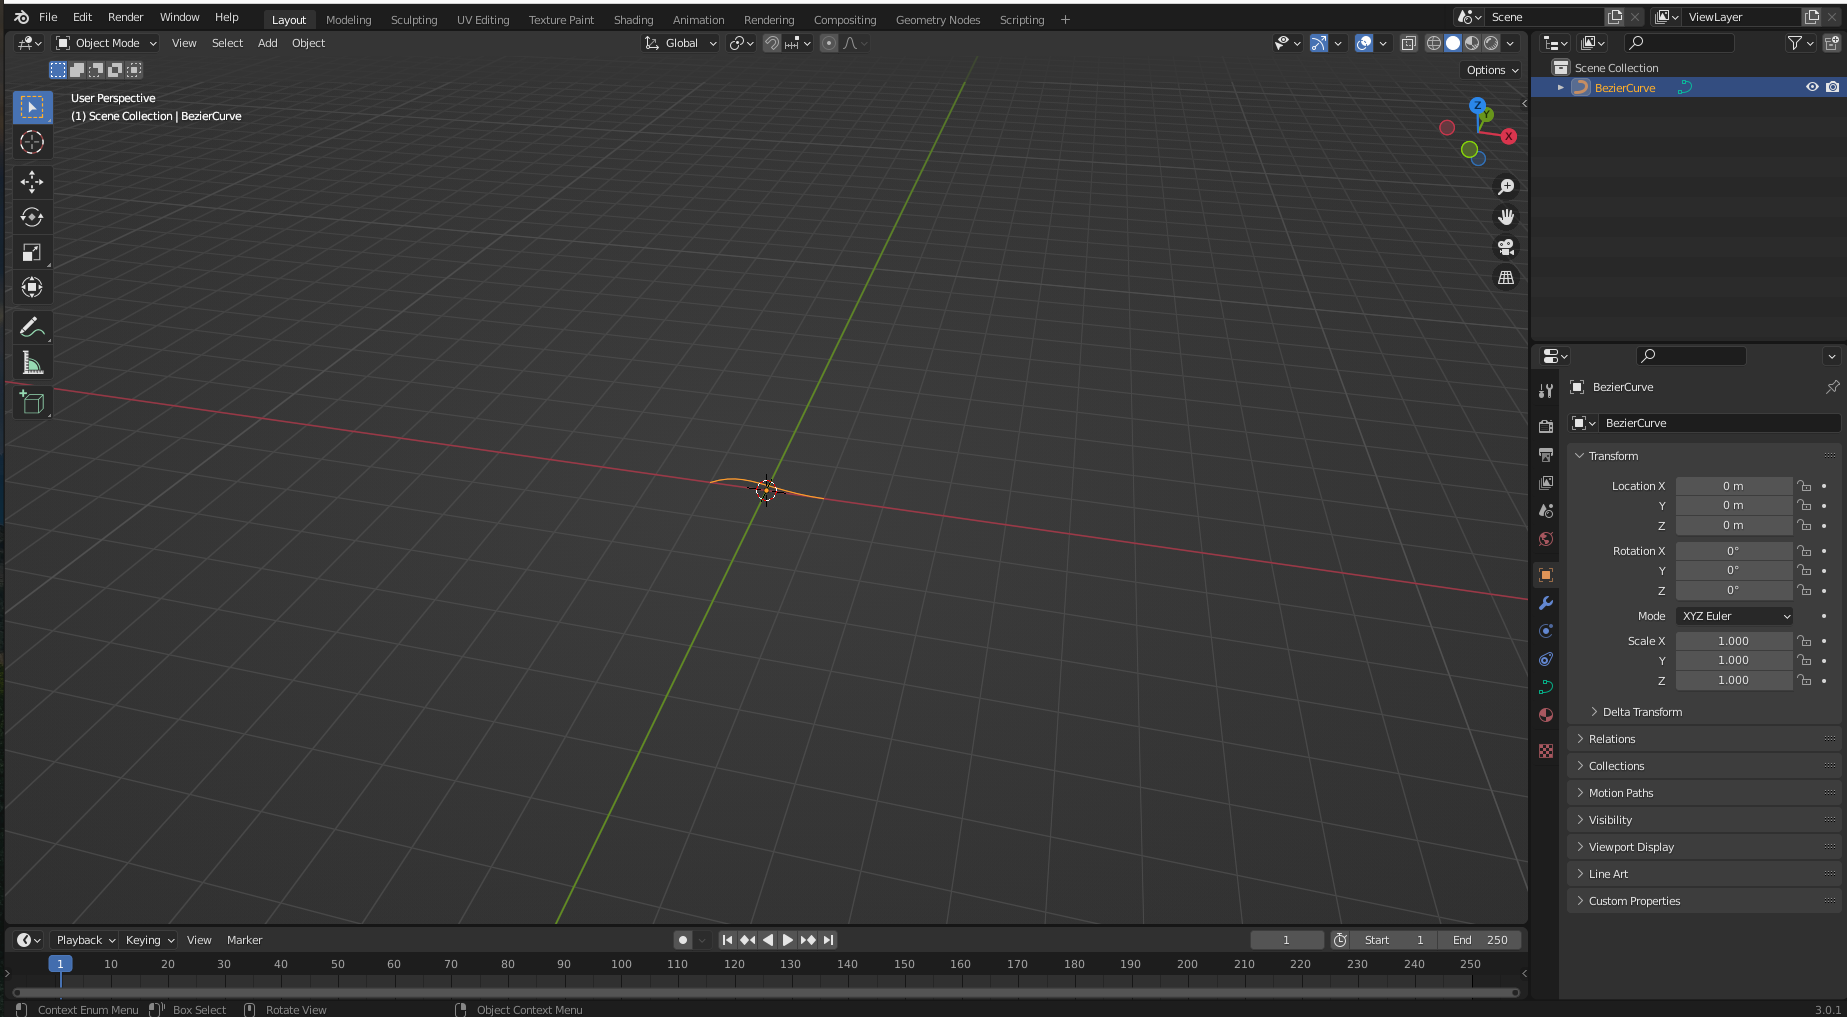
\includegraphics[width=1\linewidth]{кривая1.png}
    \label{fig:i1}
}
\vskip 1cm


\item Задание кривой необходимой формы:

Переходим в режим <<Edit mode>> нажатием табуляции  $\to $   переходим в инструмент <<Add points>>(зеленая иконка в правом нижнем углу)  $\to $ по очереди выделяем точки  нажатием на кривую и выставляем необходимые координаты для каждой точки.

В итоге получим следующую форму ломаной.
\vskip 1cm
{
    \centering
    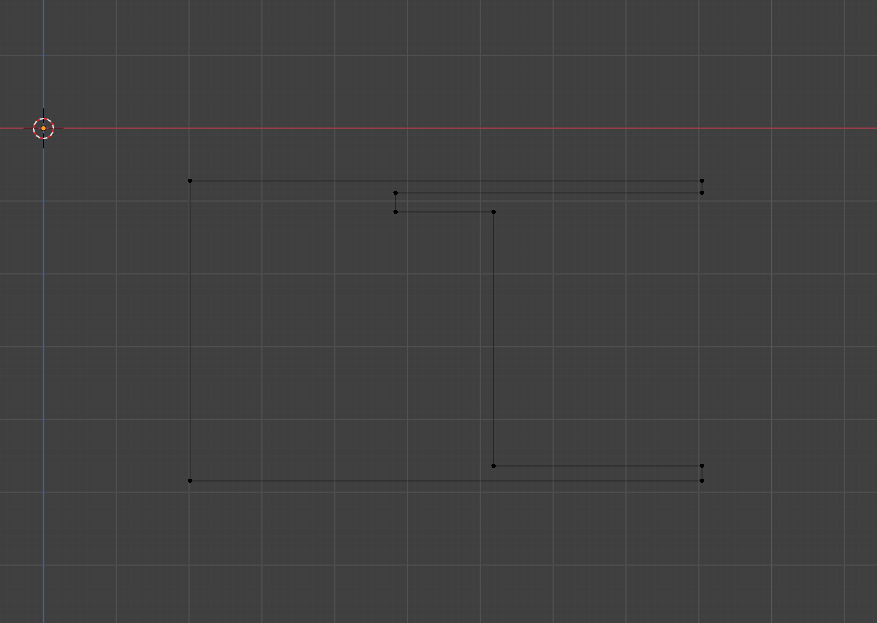
\includegraphics[width=1\linewidth]{форма_катушки.png}
    \label{fig:i1}
}
\vskip 1cm


Ниже представленны координаты в миллиметрах для каждой точки и расстановка точек на ломаной.


Расстановка точек на ломаной:

\vskip 1cm
{
    \centering
    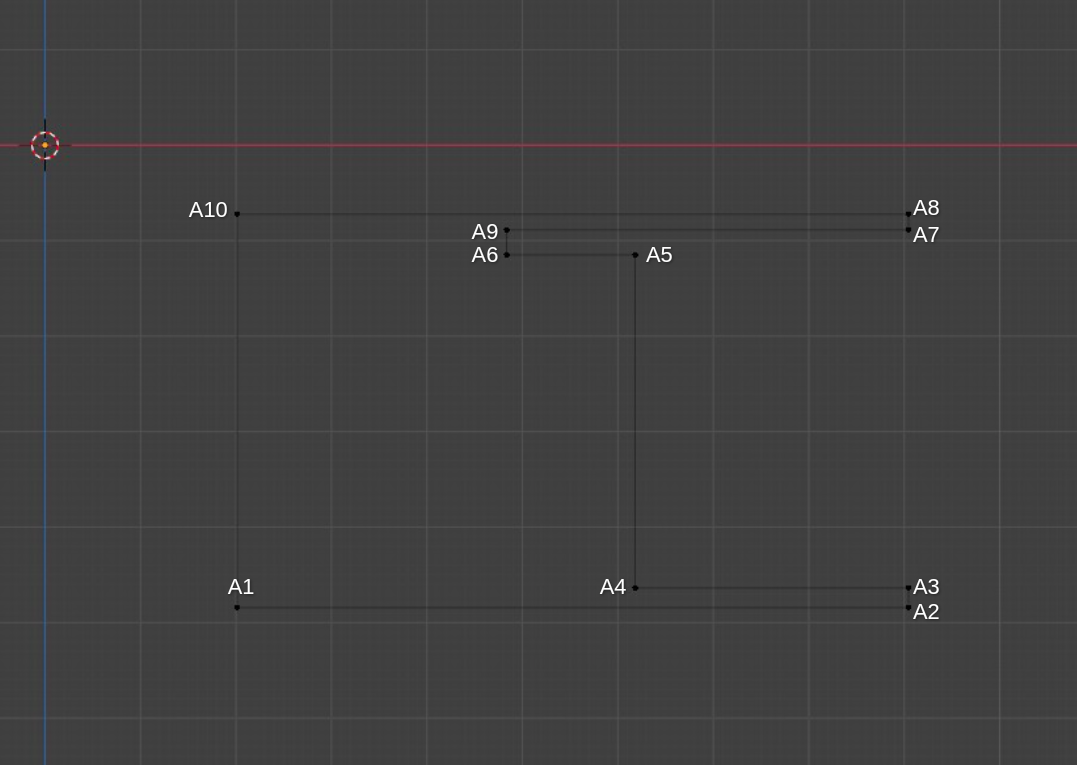
\includegraphics[width=1\linewidth]{2форма_с_точками.png}
    \label{fig:i1}
}
\vskip 1cm


Точки:

A1=\{0,0,0\};

A2=\{0,0,35\};

A3=\{1,0,35\};

A4=\{1,0,20\};

A5=\{17,0,20\};

A6=\{17,0,15\};

A7=\{19,0,35\};

A8=\{20,0,35\};

A9=\{19,0,15\};

A10=\{20,0,0\};





\item Примение модификатора <<Screw>> к кривой.

Перейти во вкладку <<Modifiers>> $\to $ нажать <<Add Modifier>>  $\to $ выбрать <<Screw>>  $\to $ изменить параметр <<Axis>> на <<Z>>(задаем ось вращения), <<angle>> - 360 $\to $  изменить <<Randor>> и <<Steps Viewport>> на 60(делаем модель более сглаженной) $\to $ нажимаем <<apply>>.



После этого на экране увидим следующее:

\vskip 1cm
{
    \centering
    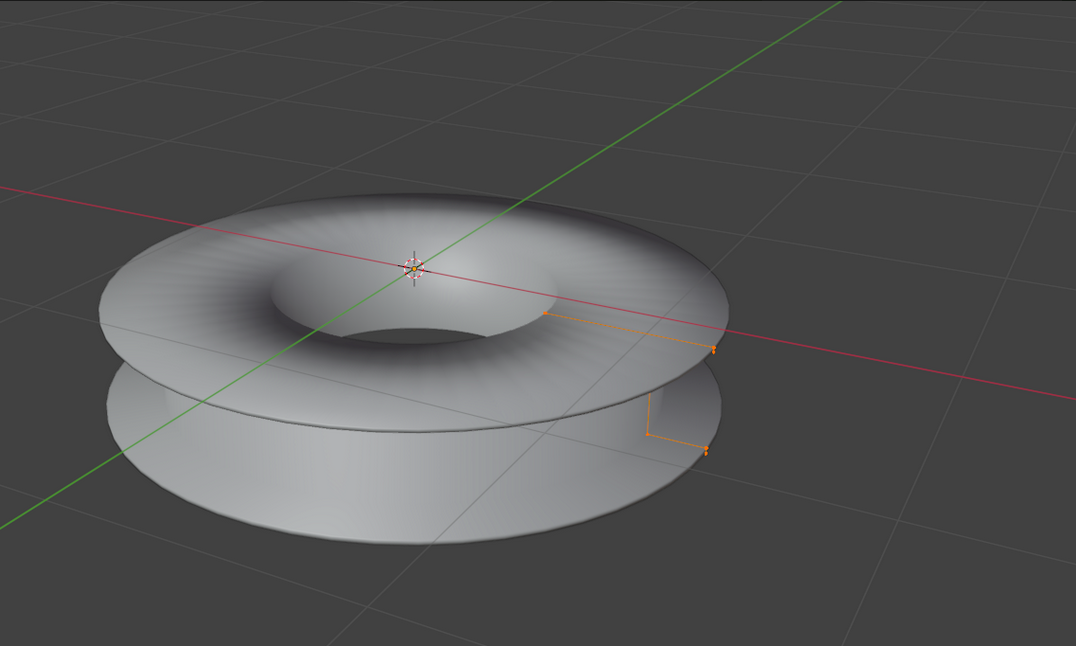
\includegraphics[width=1\linewidth]{2катушка1.png}
    \label{fig:i1}
}
\vskip 1cm


Затем нужно конвертировать объект в mesh( сетку из вершин и граней) для дальнейшего редактирования.

Нажать:<<Object>>$\to $<<convert>>$\to $<<mesh>>.




\item Модуляция деффекта на гране катушки.

Нажать Shift+пробел для открытия окна выбора инструментов $\to $ выбрать <<draw>>(рисование) $\to $ провести кривую нужной формы для выреза дефекта. 

Вид полученной кривой:

\vskip 1cm
{
    \centering
    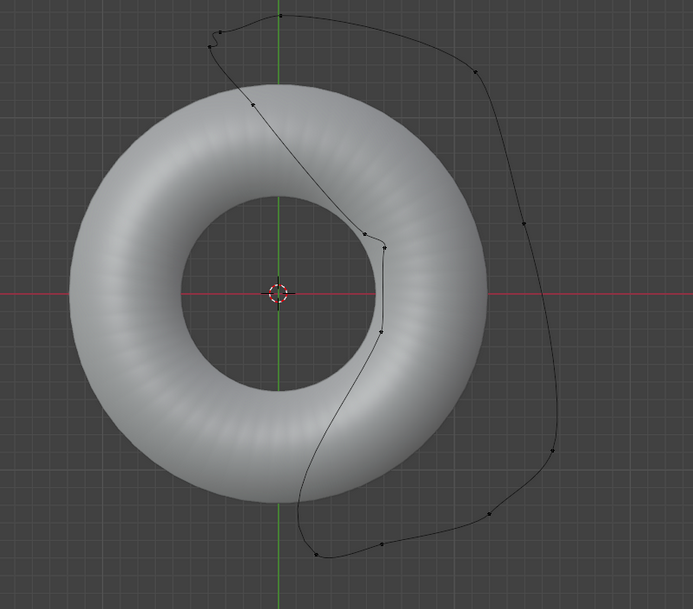
\includegraphics[width=1\linewidth]{2кривая_дефекта.png}
    \label{fig:i1}
}
\vskip 1cm


Затем нужно нажать правой кнопкой мыши и выбрать в сплывающем окне <<New face from edges>> для получения плоскости по кривой.

\item Создание объемного объекта для моделирования деффекта в основании клапана.

Перейти в инструмент <<Extrude>>  $\to $ выделить плоскость $\to $ нажать правой кнопкой мыши$\to $ выбрать поле <<Extrude region and move>> $\to $ изменить значение по оси Z на 5 mm.


Получим следующий вид модели:

\vskip 1cm
{
    \centering
    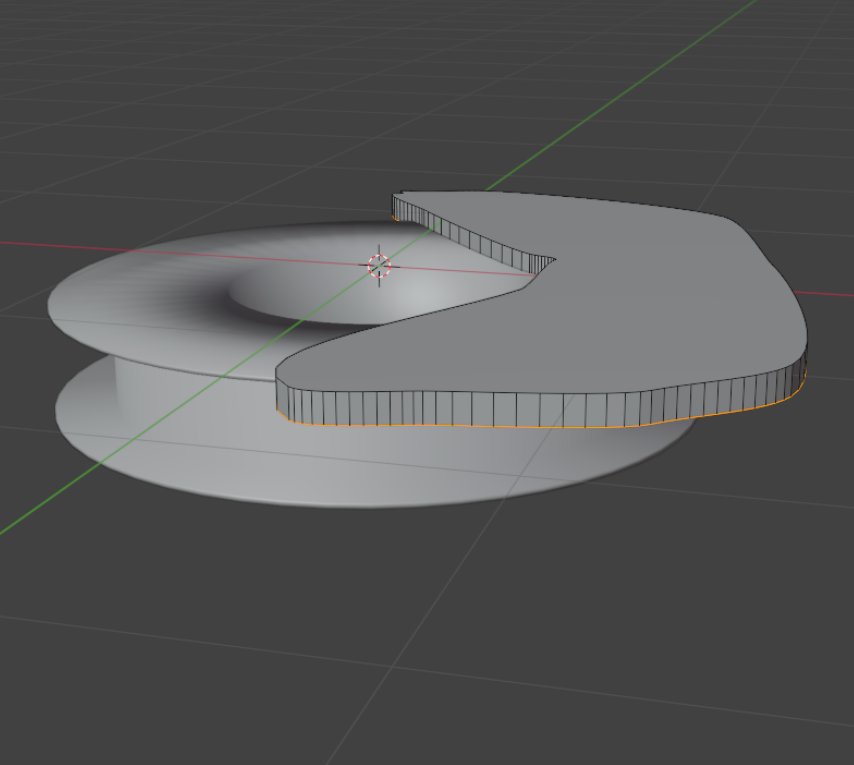
\includegraphics[width=1\linewidth]{2форма_с_диф.png}
    \label{fig:i1}
}
\vskip 1cm
	
\item Вырез области для получения дефекта модели.

Выделить основную форму $\to $ Выбрать <<Modifier properties>> на панели инструментов $\to $ в выподающем окне <<Add modifier>>  выбрать модификатор <<Boolean>> $\to $ указать параметр <<Difference>> в панеле параметров модификатора $\to $ выделить вторую модель для применения модификатора $\to $ нажать <<apply>>.

Изменим цвет модели. Для этого:


Переходим в <<Material properties>> на панели инструментов $\to $ во вкладку <<surface>> $\to $ <<Base color>> $\to $   в поле <<Set color>> выберем из представленных наиболее похожий цвет на оригинальный цвет объекта(темно-красный).


Получим следующий вид модели:

\vskip 1cm
{
    \centering
    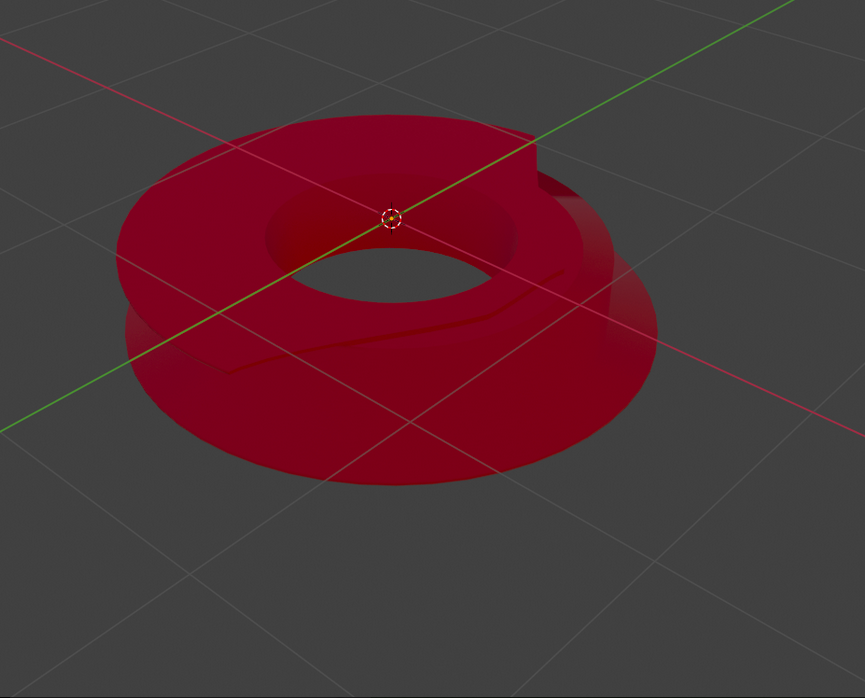
\includegraphics[width=1\linewidth]{2катушка_с_вырезом.png}
    \label{fig:i1}
}
\vskip 1cm

\item Выделение внутренней части объекта.

Перейти в режим моделирования(нажать tab) $\to $ выбрать на верхней панеле инструментов инструмент <<select>> $\to $ удерживая клавишу shift выделить нужные части на объекте  $\to $   изменим цвет для выделенных полигонов:

Переходим в <<Material properties>> на панели инструментов $\to $ во вкладку <<surface>> $\to $ <<Base color>> $\to $ в поле <<Set color>> выберем из представленных наиболее похожий цвет на оригинальный цвет объекта. Был выбран <<Purple>>.





\vskip 1cm
{
    \centering
    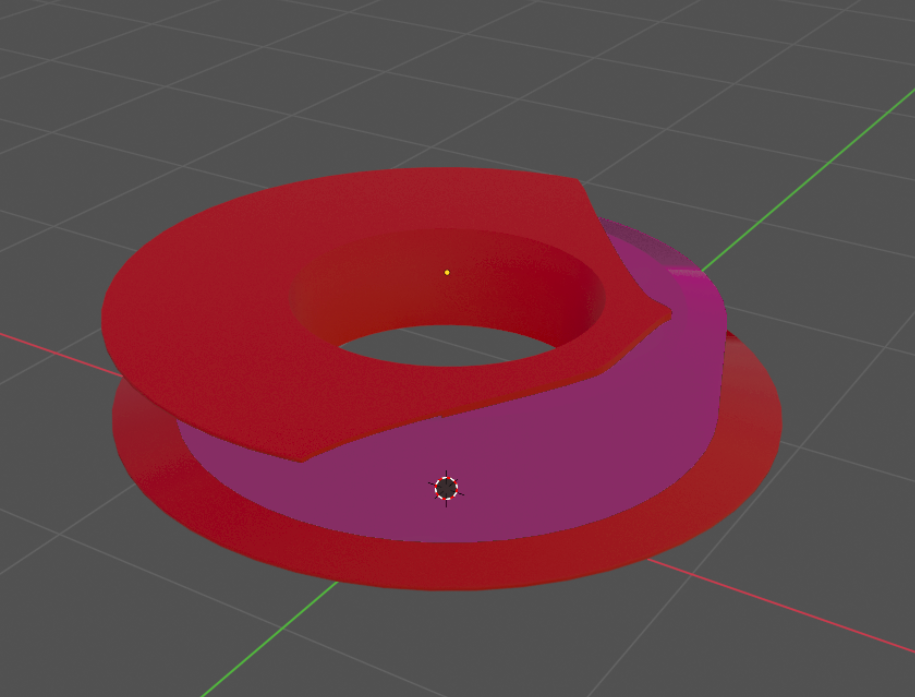
\includegraphics[width=1\linewidth]{2final.png}
    \label{fig:i1}
}
\vskip 1cm


\item Создание текстуры намотки лейкопластыря.

Находим в интернете изображение с текстурой ткани, выбираем изображение похожего цвета.


Было выбрано следующее изображение:
\vskip 1cm
{
    \centering
    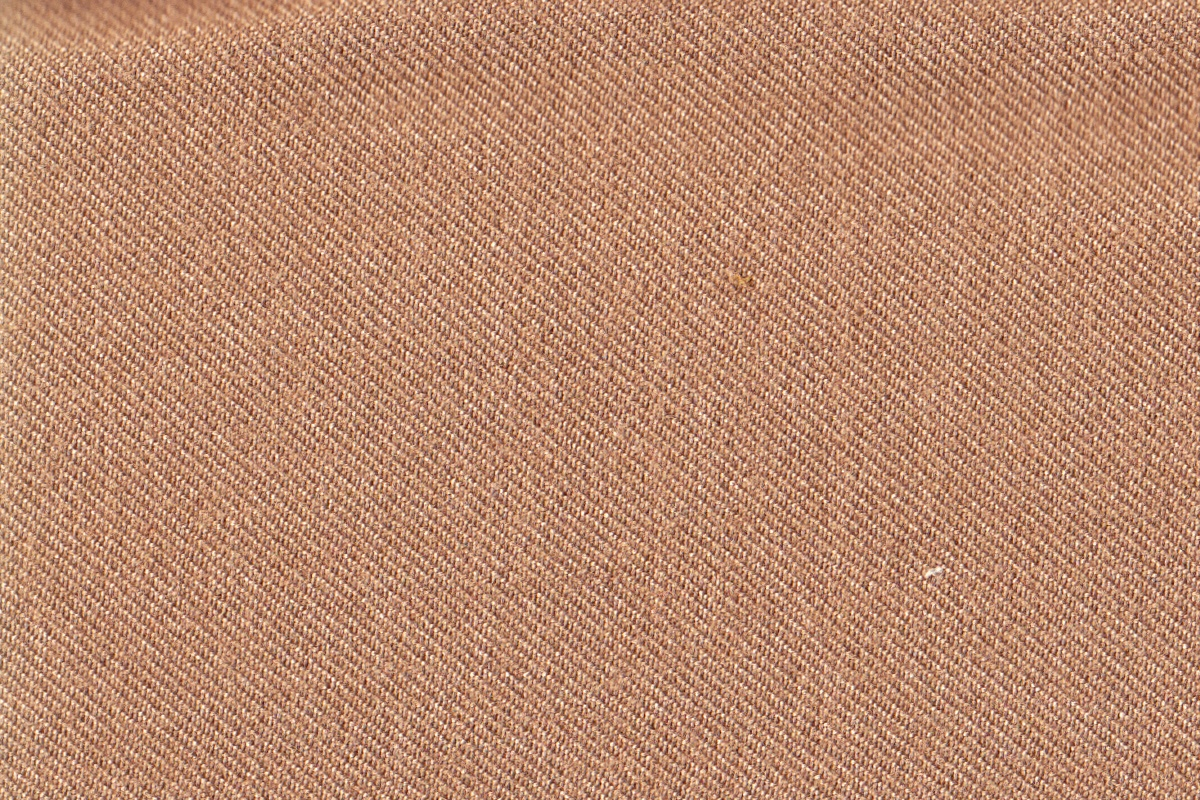
\includegraphics[width=0.6\linewidth]{текстура_пластырь.jpg}
    \label{fig:i1}
}
\vskip 1cm

Переходим во вкладку <<UV editing>>  $\to $  выделяем  горизонтальные грани для обозначения границ наложения текстуры  $\to $   Для выделения граней , выбираем их в режиме редактирования (Edit Mode) нашего объекта и используем инструменты выделения (Selection Tools) в режиме UV Editing.


Переходим во вкладку sheding  $\to $ выбираем схраненную фотографию нашей текстуры.






































Нажимаем f12 и дожидаемся окончания рендеринга.

\end{enumerate}

{\bf Результат работы:}


Финальный вид разработанной модели:

\vskip 1cm
{
    \centering
    \includegraphics[width=1\linewidth]{катушка_рендер.png}
    \label{fig:i1}
}
\vskip 1cm


\newpage


\section{Заключение}

В результате работы было сделано:


\begin{itemize}
\item  Получен навык работы с программным продуктом Blender.

\item  Были созданы трехмерные модели, повторяющие реальные объекты: Дверной ключ, клапан для воды, катушка лейкопластической ленты.

\item Для каждого объекта была создана подробная инструкция пользователя по созданию модели.
\end{itemize}




 \addcontentsline{toc}{section}{Список использованных источников}
 \newpage
\renewcommand{\refname}{Список использованных источников}
\begin{thebibliography}{99}

  

    \bibitem{source2}\href{ URL:https://elib.spbstu.ru/dl/5/tr/2021/tr21-207.pdf/download/tr21-207.pdf?ysclid=lu6a0x97yn414433657}  {Болсуновская М.В. Компьютерная графика: Blender 3D: учеб. пособие / М.В.
Болсуновская, А.А Любченкова, В.В. Ракова. – СПб., 2021. – 118 с.}
    
     

\end{thebibliography}












\end{document}